\documentclass[usenames,dvipsnames]{beamer}
%-------------------------------------------------------
% THEME SETTINGS
%-------------------------------------------------------
\usetheme[progressstyle=movingCircCnt]{Feather}
\setbeamercolor{Feather}{fg=black!30,bg=black}
\setbeamercolor{structure}{fg=black}
\setbeamercolor{block body example}{bg=black!5!white}
\setbeamercolor{block title example}{fg=white,bg=black!40!white}

\usepackage[backend=bibtex,style=alphabetic,citestyle=alphabetic-verb]{biblatex}
\usepackage{xpatch}
\usepackage{subcaption}
\usepackage{hhline}
\usepackage{xcolor}
\usepackage{todonotes}
\usepackage[all]{foreign}
\usetikzlibrary{calc}
\usepackage{adjustbox}
\usepackage{transparent}
\usetikzlibrary{arrows.meta, calc, quotes, tikzmark}


\makeatletter
\renewcommand\@makefnmark{\hbox{\@textsuperscript{\usebeamercolor[fg]{footnote mark}\usebeamerfont*{footnote mark}[\@thefnmark]}}}
\renewcommand\@makefntext[1]{\@textsuperscript{\usebeamercolor[fg]{footnote mark}\usebeamerfont*{footnote mark}[\@thefnmark]}\usebeamerfont*{footnote} #1}
\makeatother

%Modify the Title display on frame
\makeatletter
\patchcmd\beamer@@tmpl@frametitle{\insertframetitle}{{\footnotesize \insertsection~\emphColorSlide{\insertsubsection}~\\} \textbf{\insertframetitle}}{}{}
\makeatother
%Add space to the footline
\makeatletter
\patchcmd{\beamer@calculateheadfoot}{\advance\footheight by 4pt}{\advance\footheight by 8pt}{}{}
\makeatother

%NO HEAD LINE
\makeatletter
\newenvironment{noheadline}{
	\setbeamertemplate{headline}[default] {}
	\setfootline
}{}
\makeatother

%Slide with  Section title
\AtBeginSection[]{
	\begin{noheadline}
		\showCILC{true}{\begin{frame}[noframenumbering]
			\begin{center}
				\large Chapter \thesection \\
				\vspace*{1cm}
				\centering {\usebeamerfont{title} \huge\textcolor{black}{\insertsectionhead}}
				\vspace*{1cm}
			\end{center}
		\end{frame}}
	\end{noheadline}
}


\newcommand{\setfootline}{
	\setbeamercolor{footline}{fg=white,bg=black}
	\setbeamertemplate{footline}{%
		\begin{beamercolorbox}[wd=1.0\paperwidth,left,ht=2.5ex,dp=1ex]{footline}
			\usebeamerfont{section in head/foot}%
			\hspace*{3.5ex}%
			\insertshortauthor\ |\ 
			\insertshorttitle
			\insertshortsubtitle
		\end{beamercolorbox}
	}
	\addtobeamertemplate{footline}{%
		\setlength\unitlength{1ex}%
		\begin{picture}(0,0) 
		\put(125,2.5){\makebox(0,0)[bl]{
			\includegraphics[scale=0.15]{img/gulp.png}
	}}%
		\end{picture}%
	}{}
}


\DeclareCiteCommand{\footpartcite}[\mkbibfootnote]
{\usebibmacro{prenote}}
{\usebibmacro{citeindex}%
	%\mkbibbrackets{\usebibmacro{cite}}%
	%\setunit{\addnbspace}
	\printnames{labelname}%
	\setunit{\labelnamepunct}
	\printfield[citetitle]{title}%
	\newunit
	\printfield{year}}
{\addsemicolon\space}
{\usebibmacro{postnote}}

\bibliography{../Bibliography.bib}
%%% Style
% Font and layout
\newcommand*{\defemph}[1]{\ensuremath{\mathsf{#1}}}
\renewcommand*{\S}{Section}
\newcommand*{\sota}{state-of-the-art}
% Heavily used symbol style
\newcommand*{\agentstyle}[1]{{\ensuremath{\uppercase{\defemph{#1}}}}}
\newcommand*{\agentstyleMin}[1]{{\ensuremath{\lowercase{\defemph{#1}}}}}%}
\newcommand{\agent}[1]{%
  \ifstrequal{#1}{i}%
             {\ensuremath{\lowercase{\defemph{#1}}}}%
             {\ifstrequal{#1}{A}{\agentstyle{#1}}{%
\ifstrequal{#1}{a}{\agentstyle{#1}}{%
\ifstrequal{#1}{B}{\agentstyle{#1}}{%
\ifstrequal{#1}{b}{\agentstyle{#1}}{%
\ifstrequal{#1}{C}{\agentstyle{#1}}{%
\ifstrequal{#1}{c}{\agentstyle{#1}}{%
\ifstrequal{#1}{ag}{\agentstyleMin{#1}}{%
\ifstrequal{#1}{AG}{\agentstyleMin{#1}}{%
\ifstrequal{#1}{ag_1}{\agentstyleMin{#1}}{%
\ifstrequal{#1}{ag_2}{\agentstyleMin{#1}}{%
\ifstrequal{#1}{ag_i}{\agentstyleMin{#1}}{??
}}}}}}}}}}}}%
}
\newcommand*{\possarg}[2]{\ensuremath{\defemph{#1}(#2)}}
\newcommand*{\poss}[1]{\ensuremath{\defemph{#1}}}



%%% Operators, Actions and Syntax
% Epistemic logic operators
\newcommand*{\C}{\textbf{C}}
\newcommand*{\E}{\textbf{E}}
\newcommand*{\cAlpha}[1]{\ensuremath{\mathbf{C}_\alpha{#1}}}
\newcommand*{\eAlpha}[1]{\ensuremath{\mathbf{E}_\alpha{#1}}}
\newcommand*{\eAlphaIter}[2]{\ensuremath{\mathbf{E}^{#1}_\alpha{#2}}}
%\newcommand*{\initiallyC}[1]{\ensuremath{\texttt{initially\}(#1)}}
\newcommand*{\bB}[2]{\mathbf{B}_{\agent{#1}}{#2}}
\renewcommand*{\b}[1]{\ensuremath{\mathbf{B_{\agent{#1}}}}}
% Kripke operators
\newcommand*{\brel}[1]{\ensuremath{\calB_{\defemph{#1}}}}
\newcommand*{\rrel}[1]{\ensuremath{\calR_{\defemph{#1}}}}
% Actions and fluent
\newcommand*{\distract}[2]{%
\ifstrequal{#2}{}%
{\ensuremath{\mathtt{distract}(\agent{#1})}}%
{\ensuremath{\mathtt{distract}(\agent{#1})\langle\agent{#2}\rangle}}%
}
\newcommand*{\open}[1]{%
\ifstrequal{#1}{}%
{\ensuremath{\mathtt{open}}}%
{\ensuremath{\mathtt{open}\tuple{\agent{#1}}}}%
}
\newcommand*{\shout}[1]{%
\ifstrequal{#1}{}%
{\ensuremath{\mathtt{shout\_tails}}}%
{\ensuremath{\mathtt{shout\_tails}\tuple{\agent{#1}}}}%
}
\newcommand*{\signal}[2]{%
\ifstrequal{#2}{}%
{\ensuremath{\mathtt{signal}(\agent{#1})}}%
{\ensuremath{\mathtt{signal}(\agent{#1})\langle\agent{#2}\rangle}}%
}
\newcommand*{\peek}[1]{%
\ifstrequal{#1}{}%
{\ensuremath{\mathtt{peek}}}%
{\ensuremath{\mathtt{peek}\tuple{\agent{#1}}}}%
}
\newcommand*{\tell}[2]{%
\ifstrequal{#2}{}%
{\ensuremath{\mathtt{tell}(\agent{#1})}}%
{\ensuremath{\mathtt{tell}(\agent{#1})\langle\agent{#2}\rangle}}%
}
\newcommand*{\flip}[1]{%
\ifstrequal{#1}{}%
{\ensuremath{\mathtt{flip}}}%
{\ensuremath{\mathtt{flip}\tuple{\agent{#1}}}}%
}
\newcommand*{\haskey}[1]{\ensuremath{\mathtt{key}(\agent{#1})}}
\newcommand*{\opened}{\ensuremath{\mathtt{opened}}}
\newcommand*{\head}{\ensuremath{\mathtt{heads}}}
\newcommand*{\looking}[1]{\ensuremath{\mathtt{look}(\agent{#1})}}
\newcommand*{\res}[1]{\ensuremath{\defemph{caused}(\defemph{#1})}}
\newcommand*{\sensed}[2]{\ensuremath{\defemph{sensed}(\defemph{#1})[\defemph{#2}]}}
% Syntax
\newcommand*{\exec}[2]{\ensuremath{\mathbf{executable\ }\defemph{#1} \mathbf{\ if\ } #2 }}
\newcommand*{\causes}[2]{\ensuremath{\defemph{#1} \mathbf{\ causes\ } \defemph{#2} }}
\newcommand*{\determine}[2]{\ensuremath{\defemph{#1} \mathbf{\ determines\ } \defemph{#2} }}
\newcommand*{\announce}[2]{\ensuremath{\defemph{#1} \mathbf{\ announces\ } \defemph{#2} }}
\newcommand*{\initially}[1]{\ensuremath{\mathbf{intially}\ #1}}



%%% Special words
% Action languages
\newcommand*{\ourL}{\ensuremath{m\mathcal{A}^\rho}}
\newcommand*{\mAL}{\ensuremath{m\mathcal{A}^*}}
\newcommand*{\mAP}{\ensuremath{m\mathcal{A}+}}
% Multi agent epistemic
\newcommand*{\mAGep}{multi-agent epistemic}
\newcommand*{\MAGep}{Multi-agent epistemic}
\newcommand*{\ck}{common knowledge}
\newcommand*{\mep}{MEP}
% Non-well-founded set
\newcommand*{\Wf}{Well-founded}
\newcommand*{\wf}{well-founded}
\newcommand*{\Nwf}{Non-\wf}
\newcommand*{\nwf}{non-\wf}
%Possibilities & Co.
\newcommand*{\sPoss}{\ensuremath{\Phi_{\mathbf{Poss}}}}
\newcommand*{\Pos}{Possibility}
\newcommand*{\pos}{possibility}
\newcommand*{\PosS}{Possibilities}
\newcommand*{\posS}{possibilities}



%%%Special Symbols
% Languages
\newcommand*{\lAG}{\ensuremath{\mathcal{L}_{\sAG}}}
\newcommand*{\lag}{\lAG}
\newcommand*{\lagC}{\ensuremath{\lAG^{\C}}}
% Kripke structures
\newcommand*{\state}[2]{\ensuremath{(M_{\defemph{#1}},\defemph{#2})}}
\newcommand*{\posfunc}[3]{\ensuremath{\Phi_{D_{#1}}(#2,\defemph{#3})}}
\newcommand*{\trfunc}{\ensuremath{\Phi_D}}
\newcommand*{\posfull}{\ensuremath{F_{D}}}
\newcommand*{\pospartial}{\ensuremath{P_{D}}}
\newcommand*{\posoblivious}{\ensuremath{O_{D}}}
\newcommand*{\interp}[2]{\ensuremath{M_{#1}[\pi](\defemph #2)}}
% Special Sets
\newcommand*{\sAG}{\ensuremath{\mathcal{AG}}}
\newcommand*{\sAC}{\ensuremath{\mathcal{A}}}
\newcommand*{\sF}{\ensuremath{\mathcal{F}}}
\newcommand*{\sP}{\sF}
\newcommand*{\ai}{\calA\calI}
% Graph
\newcommand*{\graphG}{\ensuremath{\mathcal{G}}}
\newcommand*{\graphVE}[2]{\graphG=\textup{(}$#1, #2$\textup{)}}
% Generic
\newcommand*{\func}[3]{#1: #2 \mapsto #3}
\renewcommand*{\implies}{\ensuremath{\Rightarrow}}



%%% Shortcuts
\newcommand*{\bra}[1]{\ensuremath{\{#1\}}}
\newcommand*{\tuple}[1]{\ensuremath{\langle #1 \rangle}}



%%% Calligraphics macros by E. Zaffanella
\newcommand*{\calA}{\ensuremath{\mathcal{A}}}
\newcommand*{\calB}{\ensuremath{\mathcal{B}}}
\newcommand*{\calC}{\ensuremath{\mathcal{C}}}
\newcommand*{\calD}{\ensuremath{\mathcal{D}}}
\newcommand*{\calE}{\ensuremath{\mathcal{E}}}
\newcommand*{\calF}{\ensuremath{\mathcal{F}}}
\newcommand*{\calG}{\ensuremath{\mathcal{G}}}
\newcommand*{\calH}{\ensuremath{\mathcal{H}}}
\newcommand*{\calI}{\ensuremath{\mathcal{I}}}
\newcommand*{\calJ}{\ensuremath{\mathcal{J}}}
\newcommand*{\calK}{\ensuremath{\mathcal{K}}}
\newcommand*{\calL}{\ensuremath{\mathcal{L}}}
\newcommand*{\calM}{\ensuremath{\mathcal{M}}}
\newcommand*{\calN}{\ensuremath{\mathcal{N}}}
\newcommand*{\calO}{\ensuremath{\mathcal{O}}}
\newcommand*{\calP}{\ensuremath{\mathcal{P}}}
\newcommand*{\calQ}{\ensuremath{\mathcal{Q}}}
\newcommand*{\calR}{\ensuremath{\mathcal{R}}}
\newcommand*{\calS}{\ensuremath{\mathcal{S}}}
\newcommand*{\calT}{\ensuremath{\mathcal{T}}}
\newcommand*{\calU}{\ensuremath{\mathcal{U}}}
\newcommand*{\calV}{\ensuremath{\mathcal{V}}}
\newcommand*{\calW}{\ensuremath{\mathcal{W}}}
\newcommand*{\calX}{\ensuremath{\mathcal{X}}}
\newcommand*{\calY}{\ensuremath{\mathcal{Y}}}
\newcommand*{\calZ}{\ensuremath{\mathcal{Z}}}



%% Checkmark
\def\checkmark{\tikz\fill[scale=0.4](0,.35) -- (.25,0) -- (1,.7) -- (.25,.15) -- cycle;}

%%For SLIDES only
\newcommand*{\emphColorSlide}[1]{\textcolor{ForestGreen}{#1}}
\newcommand*{\emphSlide}[1]{\emphColorSlide{\emph{#1}}}
\newcommand*{\ttSlide}[1]{\textcolor{NavyBlue}{\texttt{#1}}}

\newcommand*{\colorAgentSlide}[1]{\textcolor{Black}{#1}}
\newcommand*{\agentSlide}[1]{%
\ifstrequal{#1}{Charlie}{\colorAgentSlide{\texttt{#1}}}%
{\ifstrequal{#1}{Lucy}{\colorAgentSlide{\texttt{#1}}}%
{\ifstrequal{#1}{Snoopy}{\colorAgentSlide{\texttt{#1}}}%
{\ifstrequal{#1}{ag}{\colorAgentSlide{\texttt{#1}}}%
{\ifstrequal{#1}{ag_i}{\ensuremath{\colorAgentSlide{\mathtt{#1}}}}%
{\ifstrequal{#1}{ag_1}{\ensuremath{\colorAgentSlide{\mathtt{#1}}}}%
{\ifstrequal{#1}{ag_2}{\ensuremath{\colorAgentSlide{\mathtt{#1}}}}%
{\ifstrequal{#1}{AG}{\colorAgentSlide{\texttt{\lowercase{#1}}}}%
{\ifstrequal{#1}{A}{\colorAgentSlide{\texttt{#1}}}%
{\ifstrequal{#1}{B}{\colorAgentSlide{\texttt{#1}}}%
{\ifstrequal{#1}{C}{\colorAgentSlide{\texttt{#1}}}%
{\ifstrequal{#1}{a}{\colorAgentSlide{\uppercase{\texttt{#1}}}}%
{\ifstrequal{#1}{b}{\colorAgentSlide{\uppercase{\texttt{#1}}}}%
{\ifstrequal{#1}{c}{\colorAgentSlide{\uppercase{\texttt{#1}}}}%
{\ifstrequal{#1}{agent}{\colorAgentSlide{\texttt{#1}}}%
{\ifstrequal{#1}{agents}{\colorAgentSlide{\texttt{#1}}}{??%
}}}}}}}}}}}}}}}}%
}
\newcommand*{\resSlide}[2]{\defemph{caused(#1)}[\ttSlide{#2}]}
\newcommand*{\sensedSlide}[2]{\defemph{sensed(#1)}[\ttSlide{#2}]}
\newcommand*{\brelSlide}[1]{\ensuremath{\calR_{\defemph{#1}}}}
\newcommand*{\bBSlide}[2]{\mathbf{B}_{\texttt{#1}}{#2}}
\newcommand{\showCILC}[2]{%
	\ifstrequal{#1}{true}{#2}{}}


%\full (Azione, pointed kripke structure(2 argomenti), insieme  )
%\newcommand*{\Interp}[2]{\ensuremath{M_{#1}[\pi](#2)}}
%\newcommand*{\nwfeq}[3]{\ensuremath{#1(#2)=#3}}


%-------------------------------------------------------
% INFORMATION IN THE TITLE PAGE
%-------------------------------------------------------

\title[] % [] is optional - is placed on the bottom of the sidebar on every slide
{ % is placed on the title page
	\textbf{
		NON-WELL-FOUNDED SET BASED MULTI-AGENT EPISTEMIC ACTION LANGUAGE}
}

\subtitle[{\color{ForestGreen}\textbf{CILC}}]
{
	{\color{ForestGreen} $\mathbf{34^{th}}$ \textbf{Italian Conference on Computational Logic}}
}

\author[\textbf{Francesco Fabiano}, Idriss Riouak, Agostino Dovier and Enrico Pontelli]
{ \textbf{Francesco Fabiano}, Idriss Riouak,\\ Agostino Dovier and Enrico Pontelli }

\institute[]
{\vspace{1cm}
	\textbf{University of Udine}\\
	\textbf{Department of Mathematics, Computer Science and Physics} \\
}

\date{\today}



\begin{document}
\setfootline
%-------------------------------------------------------
% THE TITLEPAGE
%-------------------------------------------------------

{\1
	\showCILC{true}{\begin{frame}[plain,noframenumbering]
		\titlepage
	\end{frame}}}

%-------------------------------------------------------
% BODY
%-------------------------------------------------------
\showCILC{true}{\begin{frame}{Overview}
	\setbeamertemplate{section in toc}[sections numbered]
	\setbeamertemplate{subsection in toc}{ b 
		$\ \ \ \ \ \bullet$ \inserttocsubsection \par}
	\tableofcontents
\end{frame}}




\section{Multi-Agent Epistemic Planning}
%\subsection*{Introduction}
\showCILC{true}{
	\begin{frame}{Introduction}
	\onslide<1->{
		\begin{block}{Epistemic Reasoning}
			Reasoning not only about agents' \emphSlide{perception of the world} but also about agents' \emphSlide{knowledge} and/or \emphSlide{beliefs} of her and others' beliefs.
		\end{block}
	}

	\onslide<2->{
		\begin{block}{Multi-agent Epistemic Planning Problem~\cite{bolander2011epistemic}}
			Finding \emphSlide{plans} where the goals can refer to:
			\begin{itemize}
				\item [-] the state of the world
				\item [-] the knowledge and/or the  beliefs  of the agents
			\end{itemize}
		\end{block}
	}

	\end{frame}
}

\showCILC{true}{
	\begin{frame}{An Example}
		\onslide<2->{
			\begin{exampleblock}{Initial State}
				\begin{itemize}
					\item[-] 	\agentSlide{Snoopy} and \agentSlide{Charlie} are \ttSlide{looking} while  \agentSlide{Lucy} is \ttSlide{$\neg$looking}
					\item[-] 	No one knows the \ttSlide{coin position}.
				\end{itemize}
			\end{exampleblock}
		}
		\onslide<1->{
			\centering
			\includegraphics[width=0.8\textwidth]{img/initial_state}
		}
	\end{frame}
}

\showCILC{true}{
	\begin{frame}{An Example}

		\begin{exampleblock}{Goal State}
			\begin{itemize}
				\item[-] \agentSlide{Charlie} knows the \ttSlide{coin position}\\
				\item[-] \agentSlide{Lucy} knows that \agentSlide{Charlie} knows the \ttSlide{coin position}\\
				\item[-] \agentSlide{Snoopy} does not know anything about the plan execution\\
			\end{itemize}
		\end{exampleblock}
		\centering
		\includegraphics[width=0.8\textwidth]{img/goal_state}
	\end{frame}
}


\showCILC{true}{
	\begin{frame}{Challenges}
		\begin{columns}
			\begin{column}{0.8\textwidth}
				\begin{center}
					An \agentSlide{agent} has to reason about his actions effects on
					\begin{itemize}
						\item[-] The \emphSlide{state of the world}\\
						\item[-] The \agentSlide{agents}' awareness of the environment\\
						\item[-] The \agentSlide{agents}' awareness of other \agentSlide{agents}' \emphSlide{actions}\\
						\item[-] The knowledge of other \agentSlide{agents} about his own\\
					\end{itemize}
				\end{center}
			\end{column}

			\begin{column}{0.3\textwidth}
				\centering
				\includegraphics[width=0.8\textwidth]{img/confused_charlie}
			\end{column}
		\end{columns}
	\end{frame}
}


%\subsection*{Problem Formalization}
\showCILC{true}{
	\begin{frame}{Notations}
		Given a set of \agentSlide{agents} \sAG\
		%	\onslide<1->{
		%		\begin{tikzpicture}[remember picture,overlay]
		%		\node[xshift=-5.1cm,yshift=-4cm] (A) at (current page.north east){};
		%		\node[xshift=-1.0cm,yshift=-3.5cm] (B) at (current page.north east){\NWFSGreen{Belief}};
		%		\draw[] (B)-- +(0,-0.7);
		%		\draw[to path={-| (\tikztotarget)}] (B)+(0,-0.7) edge  (A);
		%		\end{tikzpicture}%}
		\onslide<1->{

			\begin{block}{Modal operator $\bBSlide{ag}{}$ \hfill {\footnotesize where \texttt{ag} $\in$ \sAG}}
				Models the beliefs of \agentSlide{ag} about the \ttSlide{state of the world} and/or about the beliefs of other \agentSlide{agents}.
			\end{block}}
		\onslide<2->{
			\begin{block}{Group operator $\cAlpha{}$ \hfill {\footnotesize where $\alpha \subseteq$ \sAG}}
				Expresses the \emphSlide{common belief} of a group of \agentSlide{agents}.
			\end{block}}
		\onslide<3->{
			\begin{block}{Belief Formulae}
				Take into consideration \emphSlide{fluents} and/or \agentSlide{agents}' beliefs.
			\end{block}}
	\end{frame}
}

\showCILC{true}{
	\begin{frame}{Example of Belief Formulae}

		\begin{columns}
			\hspace*{0.8cm}\begin{column}{0.8\textwidth}
				Given
				\begin{itemize}
					\item[-] \sAG\ $= \{\agentSlide{Snoopy},\agentSlide{Charlie},\agentSlide{Lucy}\}$
					\item[-] \sF~~~$= \{\ttSlide{opened},\ttSlide{head},\ttSlide{looking}_{\agentSlide{ag}}\}~\agentSlide{ag} \in \sAG$
				\end{itemize}
			\end{column}
			\begin{column}{0.3\textwidth}
				\hspace*{-0.6cm}
				\includegraphics[width=1.0\textwidth]{img/initial_state}
			\end{column}
		\end{columns}
		~\newline
		\begin{exampleblock}{$\bBSlide{Snoopy}{\bBSlide{Charlie}{\neg \text{\texttt{opened}}}}$}
			\agentSlide{Snoopy} believes that \agentSlide{Charlie} believes that the box is \ttSlide{$\neg$opened}.
		\end{exampleblock}

		\onslide<2>{\begin{exampleblock}{$\cAlpha{(\neg\bBSlide{Lucy}{\mathtt{heads}} \wedge \neg \bBSlide{Lucy}{\neg \mathtt{head}})}$ \hfill {\footnotesize where $\alpha=\sAG$}}
				It is \ck\ that \agentSlide{Lucy} does not know whether the coin lies \ttSlide{heads} or \ttSlide{tails} up
			\end{exampleblock}}
	\end{frame}
}

\subsection*{}
\showCILC{true}{
	\begin{frame}{Knowledge vs. Belief}
		\begin{itemize}
			\item[-] The modal operator $\bBSlide{\agentSlide{ag}}{}$ represents the worlds' relation
			\item[-] Different relation's properties imply different meaning for $\bBSlide{\agentSlide{ag}}{}$
			      \only<2>{\item[-] \emphSlide{$\mathcal{K}$nowledge} and \emphSlide{$\mathcal{B}$elief} are characterized by a subset of the following axioms}
		\end{itemize}
		\vfill
		\only<+>{
			\begin{figure}
				\begin{subfigure}{0.5\textwidth}
					\centering
					%	\hspace*{-0.5cm}
					\includegraphics[width=0.6\textwidth]{img/sunny2}
				\end{subfigure}%
				\begin{subfigure}{0.5\textwidth}
					\centering
					%\vspace*{0.7cm}
					%\hspace*{-0.6cm}
					\includegraphics[width=0.8\textwidth]{img/flatearth}
				\end{subfigure}
			\end{figure}

		}
		\only<+>{\begin{block}{Serial (\textbf{D}) and S5 (\textbf{K,T,4,5}) Axioms}
				Given the fluent formulae $\phi$, $\psi$ and the worlds \texttt{i}, \texttt{j}
				\begin{itemize}
					\item[D] $\neg \calR_{\mathtt{i}} \bot$ \hfill  {\emphSlide{$\mathcal{B~K}$}}
					\item[K] $(\calR_{\mathtt{i}}\varphi \wedge \calR_{\mathtt{i}}(\varphi \implies \psi)) \implies  \calR_{\mathtt{i}}\psi$ \hfill {\emphSlide{$\mathcal{B~K}$}}
					\item[T] $\calR_{\mathtt{i}}\varphi  \implies \varphi$ \hfill {\emphSlide{$\mathcal{K}$}}
					\item[4] $\calR_{\mathtt{i}}\varphi  \implies \calR_{\mathtt{i}}\calR_{\mathtt{i}}\varphi$ \hfill {\emphSlide{$\mathcal{B~K}$}}
					\item[5] $\neg \calR_{\mathtt{i}}\varphi  \implies \calR_{\mathtt{i}}\neg \calR_{\mathtt{i}}\varphi$ \hfill {\emphSlide{$\mathcal{B~K}$}}
				\end{itemize}
			\end{block}}
	\end{frame}
}

%\section{Epistemic Operators}
\section{Kripke Structures}
%%%%%%%   KRIPKE STRUCTURES
\showCILC{true}{
	\begin{frame}{Description}
		\vspace{2mm}
		\showCILC{true}{
			\onslide<+->{
			\begin{block}{Pointed Kripke structure}
			A \emph{Pointed Kripke structure} is a pair (\tuple{S, \pi, \brelSlide{1},$\dots$ , \brelSlide{n}}, $s_0$), s.t.:
			\begin{itemize}
				\item[-] $S$ is a set of \emphSlide{worlds} and  $s_0 \in S$
				\item[-] $\func{\pi}{S}{2^{\sF}}$ associates an \emphSlide{interpretation} to each element of S
				\item[-] for $1 \leq \defemph{i} \leq \defemph{n}$, $\brelSlide{i} \subseteq S \times S$  is a binary relation over S
			\end{itemize}
		\end{block}
		}
	}
		\begin{columns}
			\onslide<+->{\begin{column}{0.5\textwidth}

					\vspace*{-0.1cm}\hspace*{-0.6cm}\scalebox{0.7} {

\tikzset{every picture/.style={line width=0.75pt}} %set default line width to 0.75pt        

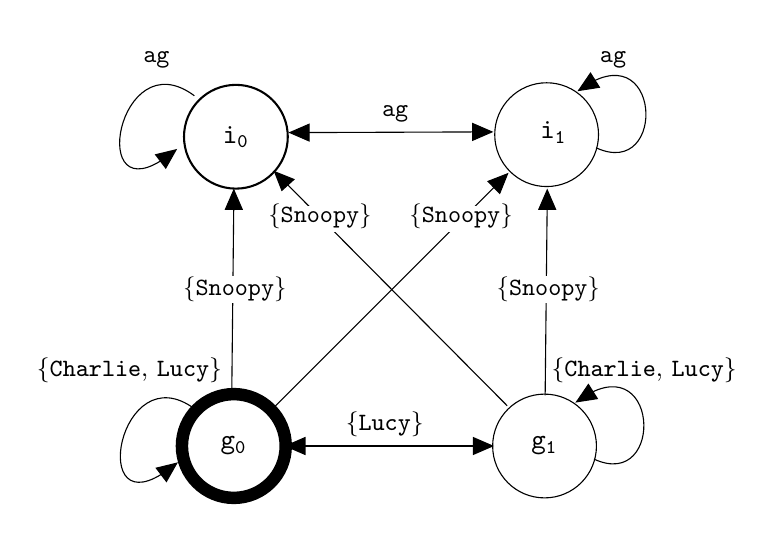
\begin{tikzpicture}[x=0.75pt,y=0.75pt,yscale=-1,xscale=1]
%uncomment if require: \path (0,300); %set diagram left start at 0, and has height of 300

%Curve Lines [id:da6922101751426857] 
\draw    (326.43,51.72) .. controls (366.43,21.72) and (369.63,95.32) .. (334.83,79.32) ;


%Curve Lines [id:da6315070066186073] 
\draw    (141.29,54.27) .. controls (104.49,26.67) and (88.76,113.08) .. (128.76,83.08) ;


%Straight Lines [id:da0043984547546391806] 
\draw    (191.92,72) -- (280.03,71.67) ;


%Straight Lines [id:da8170776057111964] 
\draw    (311.29,104.28) -- (310.29,198.64) ;


%Straight Lines [id:da10125059076875131] 
\draw    (288.88,95.12) -- (177.9,206.1) ;


%Straight Lines [id:da13591440442801073] 
\draw    (183.13,94.02) -- (292,203.6) ;


%Curve Lines [id:da0862450190271058] 
\draw    (141.62,205.27) .. controls (104.82,177.67) and (89.1,264.08) .. (129.1,234.08) ;


%Straight Lines [id:da17405321396390305] 
\draw    (160.29,104.28) -- (159.29,198.64) ;


%Straight Lines [id:da018251469869151382] 
\draw    (185.29,223) -- (285,223) ;

%Curve Lines [id:da8507870813478686] 
\draw    (325.43,201.72) .. controls (365.43,171.72) and (368.63,245.32) .. (333.83,229.32) ;

%Shape: Circle [id:dp9462184779936802] 
\draw   (286,73) .. controls (286,59.19) and (297.19,48) .. (311,48) .. controls (324.81,48) and (336,59.19) .. (336,73) .. controls (336,86.81) and (324.81,98) .. (311,98) .. controls (297.19,98) and (286,86.81) .. (286,73) -- cycle ;
%Shape: Circle [id:dp6359205424734804] 
\draw  [line width=4.5]  (135.29,223) .. controls (135.29,209.19) and (146.48,198) .. (160.29,198) .. controls (174.09,198) and (185.29,209.19) .. (185.29,223) .. controls (185.29,236.81) and (174.09,248) .. (160.29,248) .. controls (146.48,248) and (135.29,236.81) .. (135.29,223) -- cycle ;
%Shape: Circle [id:dp06782137726568571] 
%Shape: Circle [id:dp8938158972072578] 
\draw  [line width=0.75]  (135.29,223) .. controls (135.29,209.19) and (146.48,198) .. (160.29,198) .. controls (174.09,198) and (185.29,209.19) .. (185.29,223) .. controls (185.29,236.81) and (174.09,248) .. (160.29,248) .. controls (146.48,248) and (135.29,236.81) .. (135.29,223) -- cycle ;
%Shape: Circle [id:dp19780391712041556] 
\draw   (285,223) .. controls (285,209.19) and (296.19,198) .. (310,198) .. controls (323.81,198) and (335,209.19) .. (335,223) .. controls (335,236.81) and (323.81,248) .. (310,248) .. controls (296.19,248) and (285,236.81) .. (285,223) -- cycle ;
%Shape: Triangle [id:dp4725710951486233] 
\draw  [fill={rgb, 255:red, 0; green, 0; blue, 0 }  ,fill opacity=1 ] (132.8,231.28) -- (127.82,240.08) -- (122.97,233.67) -- cycle ;
%Shape: Triangle [id:dp08394946096129607] 
\draw  [fill={rgb, 255:red, 0; green, 0; blue, 0 }  ,fill opacity=1 ] (285,223) -- (275.72,227.02) -- (275.72,218.98) -- cycle ;
%Shape: Triangle [id:dp12888926826248426] 
\draw  [fill={rgb, 255:red, 0; green, 0; blue, 0 }  ,fill opacity=1 ] (185.29,223) -- (194.56,218.98) -- (194.56,227.02) -- cycle ;
%Shape: Triangle [id:dp7536519811814515] 
\draw  [fill={rgb, 255:red, 0; green, 0; blue, 0 }  ,fill opacity=1 ] (325.43,201.72) -- (331.13,193.37) -- (335.42,200.17) -- cycle ;


\draw  [line width=0.75]  (136.29,74) .. controls (136.29,60.19) and (147.48,49) .. (161.29,49) .. controls (175.09,49) and (186.29,60.19) .. (186.29,74) .. controls (186.29,87.81) and (175.09,99) .. (161.29,99) .. controls (147.48,99) and (136.29,87.81) .. (136.29,74) -- cycle ;
%Shape: Triangle [id:dp8413979641210945] 
\draw  [fill={rgb, 255:red, 0; green, 0; blue, 0 }  ,fill opacity=1 ] (132.46,80.28) -- (127.49,89.08) -- (122.64,82.67) -- cycle ;
%Shape: Triangle [id:dp417855807516911] 
\draw  [fill={rgb, 255:red, 0; green, 0; blue, 0 }  ,fill opacity=1 ] (160.29,99.64) -- (164.3,108.92) -- (156.27,108.92) -- cycle ;
%Shape: Triangle [id:dp4971926593318259] 
\draw  [fill={rgb, 255:red, 0; green, 0; blue, 0 }  ,fill opacity=1 ] (292.17,91.86) -- (288.41,101.24) -- (282.75,95.53) -- cycle ;

%Shape: Triangle [id:dp5745677700051097] 
\draw  [fill={rgb, 255:red, 0; green, 0; blue, 0 }  ,fill opacity=1 ] (326.43,51.72) -- (332.13,43.37) -- (336.42,50.17) -- cycle ;

%Shape: Triangle [id:dp7023350686012408] 
\draw  [fill={rgb, 255:red, 0; green, 0; blue, 0 }  ,fill opacity=1 ] (284.67,71.67) -- (275.39,75.69) -- (275.39,67.65) -- cycle ;
%Shape: Triangle [id:dp6039108674849356] 
\draw  [fill={rgb, 255:red, 0; green, 0; blue, 0 }  ,fill opacity=1 ] (187.29,72) -- (196.56,67.98) -- (196.56,76.02) -- cycle ;
%Shape: Triangle [id:dp9176823524690971] 
\draw  [fill={rgb, 255:red, 0; green, 0; blue, 0 }  ,fill opacity=1 ] (179.93,90.84) -- (189.24,94.56) -- (183.44,99.82) -- cycle ;
%Shape: Rectangle [id:dp7039913742222839] 
\draw  [color={rgb, 255:red, 0; green, 0; blue, 0 }  ,draw opacity=0 ][fill={rgb, 255:red, 255; green, 255; blue, 255 }  ,fill opacity=1 ] (148.29,141.18) -- (173.29,141.18) -- (173.29,153.97) -- (148.29,153.97) -- cycle ;
%Shape: Triangle [id:dp2216172811102144] 
\draw  [fill={rgb, 255:red, 0; green, 0; blue, 0 }  ,fill opacity=1 ] (311.29,99.64) -- (315.3,108.92) -- (307.27,108.92) -- cycle ;
%Shape: Rectangle [id:dp8761718319086598] 
\draw  [color={rgb, 255:red, 0; green, 0; blue, 0 }  ,draw opacity=0 ][fill={rgb, 255:red, 255; green, 255; blue, 255 }  ,fill opacity=1 ] (299.29,141.18) -- (324.29,141.18) -- (324.29,153.97) -- (299.29,153.97) -- cycle ;
%Shape: Rectangle [id:dp30238976789343086] 
\draw  [color={rgb, 255:red, 0; green, 0; blue, 0 }  ,draw opacity=0 ][fill={rgb, 255:red, 255; green, 255; blue, 255 }  ,fill opacity=1 ] (257.29,107.18) -- (282.29,107.18) -- (282.29,119.97) -- (257.29,119.97) -- cycle ;
%Shape: Rectangle [id:dp8647257034518798] 
\draw  [color={rgb, 255:red, 0; green, 0; blue, 0 }  ,draw opacity=0 ][fill={rgb, 255:red, 255; green, 255; blue, 255 }  ,fill opacity=1 ] (189.29,107.18) -- (214.29,107.18) -- (214.29,119.97) -- (189.29,119.97) -- cycle ;

% Text Node
\draw (160.29,223) node  [align=left] {$\mathtt{g_0}$};
% Text Node
\draw (310,223) node  [align=left] {$\mathtt{g_1}$};
% Text Node
\draw (161.29,74) node  [align=left] {$\mathtt{i_0}$};
% Text Node
\draw (314.29,72) node  [align=left] {$\mathtt{i_1}$};
% Text Node
\draw (238,63) node [scale=0.9] [align=left] {\agentSlide{AG}};
% Text Node
\draw (123,37) node [scale=0.9] [align=left] {\agentSlide{AG}};
% Text Node
\draw (343,37) node [scale=0.9] [align=left] {\agentSlide{AG}};
% Text Node
\draw (160.79,147.58) node [scale=0.9] [align=left] {\{\agentSlide{Snoopy}\}};
% Text Node
\draw (311.79,147.58) node [scale=0.9] [align=left] {\{\agentSlide{Snoopy}\}};
% Text Node
\draw (269.79,112.18) node [scale=0.9] [align=left] {\{\agentSlide{Snoopy}\}};
% Text Node
\draw (201.79,112.18) node [scale=0.9] [align=left] {\{\agentSlide{Snoopy}\}};
% Text Node
\draw (110,186.6) node  [align=left] {{\small \{\agentSlide{Charlie}, \agentSlide{Lucy}\}}};
% Text Node
\draw (358,186.6) node  [align=left] {{\small \{\agentSlide{Charlie}, \agentSlide{Lucy}\}}};
% Text Node
\draw (233,212.6) node  [align=left] {{\small \{\agentSlide{Lucy}\}}};
% Text Node
%\draw (230,33.07) node [scale=0.9] [align=left] {\agentSlide{AG} = \{\agentSlide{Charlie}, \agentSlide{Lucy}, \agentSlide{Snoopy}\}};


\end{tikzpicture}}

				\end{column}
				\begin{column}{0.5\textwidth}

					{\small \vspace*{-1cm}\agentSlide{AG} = \{\agentSlide{Charlie}, \agentSlide{Lucy}, \agentSlide{Snoopy}\}}

					\hspace*{-0.5cm}\includegraphics[width=1\textwidth]{img/goal_state}
				\end{column}}
		\end{columns}

	\end{frame}
}

\showCILC{true}{
	\begin{frame}{Entailment}
		Let $\varphi$ be a belief formula and \state{}{s} be a pointed Kripke structure:
		\begin{block}{Entailment w.r.t. a pointed Kripke structure}
			\begin{itemize}[<+->]
				\item[-] $\state{}{s} \models \varphi$ if $\varphi$ is a \emphSlide{fluent formula} and $\pi(\defemph{s})
					      \models \varphi$;
				\item[-] $\state{}{s} \models \mathbf{B}_{\agentSlide{ag_i}}\varphi$ if $\forall $ \defemph{t}:
				      $\defemph{(s,t)} \in \brelSlide{i}$ it holds that\ $ \state{}{t} \models \varphi$;
				      %\item $\state{}{s} \models \neg \varphi$ if $\state{}{s} \not\models \varphi$;
				      %\item $\state{}{s} \models \varphi_1 \vee \varphi_2$ if $\state{}{s}\models
				      %\varphi_1$ or $\state{}{s}\models \varphi_2$;
				      %\item $\state{}{s} \models \varphi_1 \wedge \varphi_2$ if $\state{}{s}\models
				      %\varphi_1$ and $\state{}{s}\models \varphi_2$;
				\item[-] $\state{}{s} \models \eAlpha{\varphi}$ if $\state{}{s} \models
					      \mathbf{B}_{\agentSlide{ag_i}}{\varphi}$ for all \agentSlide{ag_i} $\in \alpha$;
				\item<.->[-] $\state{}{s} \models \cAlpha{\varphi}$ if
				      $\state{}{s} \models \eAlphaIter{k}{\varphi}$ for every
				      $k\geq0$, where $\eAlphaIter{0}{\varphi} = \varphi$ and
				      $\eAlphaIter{k+1}{\varphi} =\eAlpha{(\eAlphaIter{k}{\varphi})}$.
			\end{itemize}
		\end{block}
		\onslide<3->{The entailment for the standard operators is defined as usual}
	\end{frame}
}

\showCILC{false}{
	\begin{frame}{A little note on Complexity}

		\only<1>{Given a Kripke Structure $M$, a belief formula $\varphi$ and a group of agents \sAG\ s.t. $|\sAG| \geq 2$
			\begin{block}{Model-checking problem~\cite{fagin1994reasoning}}

				\begin{table}
					\def\arraystretch{1.2}%
					\begin{tabular}{||c|c|c||}
						\hhline{|t:===:t|}
						\multicolumn{1}{||c|}{\phantom{...}$\calK_1$ and $\calB_1$\phantom{...}}
						 & \multicolumn{1}{c|}{\phantom{...}$\calK_{\sAG}$ and $\calB_{\sAG}$\phantom{...}}
						 & \multicolumn{1}{c||}{\phantom{...}$\calK_{\sAG}^{\mathbf{C}}$ and $\calB_{\sAG}^{\mathbf{C}}$\phantom{...}} \\
						\hhline{||-|-|-||}
						\multicolumn{3}{||c||}{Polynomial Time -- $\mathcal{O}(||M|| \times |\varphi|)$}                               \\
						\hhline{|b:===:b|}
					\end{tabular}
				\end{table}
				{\small
				where $||M|| = |M[S]| + \sum_{i=0}^{n} |\calR_i|$}
			\end{block}
		}
		\only<2>{Given a group of agents \sAG\ s.t. $|\sAG| \geq 2$
			\begin{block}{Satisfiability problem for $\calK$nowledge and $\calB$elief~\cite{fagin1994reasoning}}
				\begin{table}
					\def\arraystretch{1.2}%
					\begin{tabular}{||c|c|c||}
						\hhline{|t:===:t|}
						\multicolumn{1}{||c|}{\phantom{...}$\calK_1$ and $\calB_1$\phantom{...}}
						 & \multicolumn{1}{c|}{\phantom{...}$\calK_{\sAG}$ and $\calB_{\sAG}$\phantom{...}}
						 & \multicolumn{1}{c||}{\phantom{...}$\calK_{\sAG}^{\mathbf{C}}$ and $\calB_{\sAG}^{\mathbf{C}}$\phantom{...}} \\
						\hhline{||-|-|-||}
						\multicolumn{1}{||c|}{NP-complete}
						 & \multicolumn{1}{c|}{PSPACE-complete}
						 & \multicolumn{1}{c||}{EXPTIME-complete}                                                                      \\
						\hhline{|b:===:b|}
					\end{tabular}
				\end{table}
				{\small w.r.t. a belief formula $\varphi$}
			\end{block}
		}
		\only<3>{

			\begin{block}{Problems in \emphSlide{DEL} without restrictions~\cite{bolander2015complexity}}
				\begin{table}
					\def\arraystretch{1.2}%
					\begin{tabular}{||c|c|c||}
						\hhline{|t:===:t|}
						\multicolumn{1}{||c|}{Model checking}
						 & \multicolumn{1}{c|}{Plan Verification Problem}
						 & \multicolumn{1}{c||}{Plan Existence}           \\
						\hhline{||-|-|-||}
						\multicolumn{1}{||c|}{PSPACE-hard}
						 & \multicolumn{1}{c|}{PSPACE-complete}
						 & \multicolumn{1}{c||}{UNDECIDABLE}                 \\
						\hhline{|b:===:b|}
					\end{tabular}
				\end{table}
				We intend to explore the last two cases with DEL restricted to $\calK$ and $\calB$
			\end{block}
		}
	\end{frame}
}

\showCILC{true}{
	\begin{frame}{Problems}
		\vspace*{0.5cm}
		\begin{columns}
			\begin{column}{0.9\textwidth}
				\begin{center}
					\begin{itemize}
						\item[-] Solvers require high amount of memory
						\item[-] In literature the states have been represented	explicitly
						\item[-] State comparison needs to find \emphSlide{bisimilar} states
					\end{itemize}
				\end{center}
			\end{column}
			\begin{column}{0.2\textwidth}
				\centering
				\includegraphics[width=0.5\textwidth]{img/worried_charlie}
			\end{column}
		\end{columns}
		\vspace*{0.5cm}
		\begin{figure}
			\centering
			\scalebox{.45}{\input{img/equality1_corr}}
			\scalebox{.45}{\tikzset{every picture/.style={line width=0.75pt}} %set default line width to 0.75pt        
\trimbox{0cm 0cm 0cm 1.8cm}{ 
\begin{tikzpicture}[x=0.75pt,y=0.75pt,yscale=-1,xscale=1]
%uncomment if require: \path (0,332); %set diagram left start at 0, and has height of 332

%Shape: Circle [id:dp09506861109760789] 
\draw   (67.5,279.5) .. controls (67.5,262.66) and (81.16,249) .. (98,249) .. controls (114.84,249) and (128.5,262.66) .. (128.5,279.5) .. controls (128.5,296.34) and (114.84,310) .. (98,310) .. controls (81.16,310) and (67.5,296.34) .. (67.5,279.5) -- cycle ;
%Shape: Circle [id:dp3674876277032001] 
\draw   (240.5,279.5) .. controls (240.5,262.66) and (254.16,249) .. (271,249) .. controls (287.84,249) and (301.5,262.66) .. (301.5,279.5) .. controls (301.5,296.34) and (287.84,310) .. (271,310) .. controls (254.16,310) and (240.5,296.34) .. (240.5,279.5) -- cycle ;
%Straight Lines [id:da686791560478396] 
\draw    (131,279.5) -- (238.5,279.5) ;
\draw [shift={(240.5,279.5)}, rotate = 180] [fill={rgb, 255:red, 0; green, 0; blue, 0 }  ][line width=0.75]  [draw opacity=0] (8.93,-4.29) -- (0,0) -- (8.93,4.29) -- cycle    ;
\draw [shift={(129,279.5)}, rotate = 0] [fill={rgb, 255:red, 0; green, 0; blue, 0 }  ][line width=0.75]  [draw opacity=0] (8.93,-4.29) -- (0,0) -- (8.93,4.29) -- cycle    ;
%Curve Lines [id:da3133467592132765] 
\draw    (67.5,279.5) .. controls (-31.5,263.58) and (50.67,180.83) .. (89.42,247.48) ;
\draw [shift={(90,248.5)}, rotate = 240.66] [fill={rgb, 255:red, 0; green, 0; blue, 0 }  ][line width=0.75]  [draw opacity=0] (8.93,-4.29) -- (0,0) -- (8.93,4.29) -- cycle    ;

%Curve Lines [id:da09866336174690571] 
\draw    (301.5,279.5) .. controls (391.91,267.58) and (313.16,179.07) .. (280.98,249.43) ;
\draw [shift={(280.5,250.5)}, rotate = 293.78] [fill={rgb, 255:red, 0; green, 0; blue, 0 }  ][line width=0.75]  [draw opacity=0] (8.93,-4.29) -- (0,0) -- (8.93,4.29) -- cycle    ;

%Shape: Circle [id:dp9019764791073822] 
\draw  [fill={rgb, 255:red, 0; green, 0; blue, 0 }  ,fill opacity=1 ] (240.5,73.5) .. controls (240.5,56.66) and (254.16,43) .. (271,43) .. controls (287.84,43) and (301.5,56.66) .. (301.5,73.5) .. controls (301.5,90.34) and (287.84,104) .. (271,104) .. controls (254.16,104) and (240.5,90.34) .. (240.5,73.5) -- cycle ;
%Shape: Circle [id:dp23164546006052256] 
\draw  [fill={rgb, 255:red, 255; green, 255; blue, 255 }  ,fill opacity=1 ] (246,73.5) .. controls (246,59.69) and (257.19,48.5) .. (271,48.5) .. controls (284.81,48.5) and (296,59.69) .. (296,73.5) .. controls (296,87.31) and (284.81,98.5) .. (271,98.5) .. controls (257.19,98.5) and (246,87.31) .. (246,73.5) -- cycle ;
%Straight Lines [id:da3406951202857561] 
\draw    (255.5,96.5) -- (112.48,251.28) ;
\draw [shift={(111.13,252.75)}, rotate = 312.74] [fill={rgb, 255:red, 0; green, 0; blue, 0 }  ][line width=0.75]  [draw opacity=0] (8.93,-4.29) -- (0,0) -- (8.93,4.29) -- cycle    ;

%Straight Lines [id:da5969218919849798] 
\draw    (271,104) -- (271,247) ;
\draw [shift={(271,249)}, rotate = 270] [fill={rgb, 255:red, 0; green, 0; blue, 0 }  ][line width=0.75]  [draw opacity=0] (8.93,-4.29) -- (0,0) -- (8.93,4.29) -- cycle    ;

%Curve Lines [id:da32162073734028385] 
\draw    (296.5,72.5) .. controls (386.91,60.58) and (308.16,-27.93) .. (275.98,42.43) ;
\draw [shift={(275.5,43.5)}, rotate = 293.78] [fill={rgb, 255:red, 0; green, 0; blue, 0 }  ][line width=0.75]  [draw opacity=0] (8.93,-4.29) -- (0,0) -- (8.93,4.29) -- cycle    ;


% Text Node
\draw  [color={rgb, 255:red, 255; green, 255; blue, 255 }  ,draw opacity=1 ][fill={rgb, 255:red, 255; green, 255; blue, 255 }  ,fill opacity=1 ]  (155.75,267.5) -- (213.75,267.5) -- (213.75,291.5) -- (155.75,291.5) -- cycle  ;
\draw (184.75,279.5) node   {\{\agentSlide{A},\agentSlide{B},\agentSlide{C}\}};
% Text Node
\draw (98,279.5) node   {\defemph{s_{0}}};
% Text Node
\draw (271,279.5) node   {\defemph{s_{1}}};
% Text Node
\draw  [color={rgb, 255:red, 255; green, 255; blue, 255 }  ,draw opacity=1 ][fill={rgb, 255:red, 255; green, 255; blue, 255 }  ,fill opacity=1 ]  (16,219.5) -- (74,219.5) -- (74,243.5) -- (16,243.5) -- cycle  ;
\draw (45,231.5) node   {\{\agentSlide{A},\agentSlide{B},\agentSlide{C}\}};
% Text Node
\draw  [color={rgb, 255:red, 255; green, 255; blue, 255 }  ,draw opacity=1 ][fill={rgb, 255:red, 255; green, 255; blue, 255 }  ,fill opacity=1 ]  (290,214.5) -- (348,214.5) -- (348,238.5) -- (290,238.5) -- cycle  ;
\draw (319,226.5) node   {\{\agentSlide{A},\agentSlide{B},\agentSlide{C}\}};
% Text Node
\draw (271,73.5) node   {\defemph{r_{1}}};
% Text Node
\draw  [color={rgb, 255:red, 255; green, 255; blue, 255 }  ,draw opacity=1 ][fill={rgb, 255:red, 255; green, 255; blue, 255 }  ,fill opacity=1 ]  (217.5,112.5) -- (238.5,112.5) -- (238.5,136.5) -- (217.5,136.5) -- cycle  ;
\draw (228,124.5) node   {\{\agentSlide{A}\}};
% Text Node
\draw  [color={rgb, 255:red, 255; green, 255; blue, 255 }  ,draw opacity=1 ][fill={rgb, 255:red, 255; green, 255; blue, 255 }  ,fill opacity=1 ]  (261,130.5) -- (282,130.5) -- (282,154.5) -- (261,154.5) -- cycle  ;
\draw (271.5,142.5) node   {\{\agentSlide{A}\}};
% Text Node
\draw  [color={rgb, 255:red, 255; green, 255; blue, 255 }  ,draw opacity=1 ][fill={rgb, 255:red, 255; green, 255; blue, 255 }  ,fill opacity=1 ]  (321,22.5) -- (359,22.5) -- (359,46.5) -- (321,46.5) -- cycle  ;
\draw (340,34.5) node   {\{\agentSlide{B},\agentSlide{C}\}};


\end{tikzpicture}}}
		\end{figure}
	\end{frame}
}


\showCILC{true}{
	\begin{frame}{Solutions}
		\begin{columns}
			\begin{column}{0.9\textwidth}
				\begin{center}
					\begin{itemize}
						\onslide<1->{\item[-] Heuristics~\cite{le2018efp}}
						      \onslide<2->{\item[-] Symbolic representation of Kripke structures %(\eg \textit{OBDDs})
						      }
						      \onslide<3>{\item[\huge \emphColorSlide{-}]\Large \emphColorSlide{Alternative representations}}
					\end{itemize}
				\end{center}
			\end{column}
			\begin{column}{0.2\textwidth}
				\centering
				\hspace*{-1cm}\includegraphics[width=1\textwidth]{img/idea_charlie}
			\end{column}
		\end{columns}

	\end{frame}
}


\section{\PosS}
%%%%%%%%%% POSSIBILITIES
\showCILC{true}{
	\begin{frame}{Overview}
		\begin{itemize}
			\item[-] Introduced by Gerbrandy and Groeneveld~\cite{Gerbrandy1997}
			\item[-] Used to represent \emphSlide{multi-agent information change}
			\item[-] Based on \emphSlide{\nwf\ sets}
			\item[-] Corresponds with a class of bisimilar Kripke structures~\cite{gerbrandy1999bisimulations}
		\end{itemize}
	\end{frame}
}

%%%%%%%%%% NWFSs
\showCILC{true}{
	\subsection*{\Nwf\ sets theory}
}

%\showCILC{true}{\begin{frame}{\Wf\ sets}
%		\begin{block}{\Wf\ set}
%			Let $E$ be a set, $E^\prime$ one of its elements, $E^{\prime\prime}$ any element of $E^\prime$, and so on. A descent is the sequence of steps from $E$ to $E^\prime$, $E^\prime$ to $E^{\prime\prime}$, etc.  A set is 
%			\alert{\wf}\ (or \emph{ordinary}) when it only gives rise to \emph{finite} descents.
%		\end{block}
%	
%	\vspace{-0.3cm}
%		\begin{figure}
%			{\scalebox{0.6}{

\tikzset{every picture/.style={line width=0.75pt}} %set default line width to 0.75pt        

\begin{tikzpicture}[x=0.75pt,y=0.75pt,yscale=-0.7,xscale=0.7]
%uncomment if require: \path (0,243); %set diagram left start at 0, and has height of 243

%Straight Lines [id:da42363008311855377] 
\draw    (126.5,47) ;
\draw [shift={(126.5,47)}, rotate = 0] [color={rgb, 255:red, 0; green, 0; blue, 0 }  ][fill={rgb, 255:red, 0; green, 0; blue, 0 }  ][line width=0.75]      (0, 0) circle [x radius= 3.35, y radius= 3.35]   ;

%Straight Lines [id:da9776475110732991] 
\draw    (196.5,47) -- (196.5,111) ;
\draw [shift={(196.5,111)}, rotate = 90] [color={rgb, 255:red, 0; green, 0; blue, 0 }  ][fill={rgb, 255:red, 0; green, 0; blue, 0 }  ][line width=0.75]      (0, 0) circle [x radius= 3.35, y radius= 3.35]   ;
\draw [shift={(196.5,47)}, rotate = 90] [color={rgb, 255:red, 0; green, 0; blue, 0 }  ][fill={rgb, 255:red, 0; green, 0; blue, 0 }  ][line width=0.75]      (0, 0) circle [x radius= 3.35, y radius= 3.35]   ;
%Straight Lines [id:da161306486001776] 
\draw    (300.5,47) -- (274.5,110) ;
\draw [shift={(274.5,110)}, rotate = 112.43] [color={rgb, 255:red, 0; green, 0; blue, 0 }  ][fill={rgb, 255:red, 0; green, 0; blue, 0 }  ][line width=0.75]      (0, 0) circle [x radius= 3.35, y radius= 3.35]   ;
\draw [shift={(300.5,47)}, rotate = 112.43] [color={rgb, 255:red, 0; green, 0; blue, 0 }  ][fill={rgb, 255:red, 0; green, 0; blue, 0 }  ][line width=0.75]      (0, 0) circle [x radius= 3.35, y radius= 3.35]   ;
%Straight Lines [id:da12831723727076116] 
\draw    (300.5,47) -- (323.5,110) ;
\draw [shift={(323.5,110)}, rotate = 69.94] [color={rgb, 255:red, 0; green, 0; blue, 0 }  ][fill={rgb, 255:red, 0; green, 0; blue, 0 }  ][line width=0.75]      (0, 0) circle [x radius= 3.35, y radius= 3.35]   ;
\draw [shift={(300.5,47)}, rotate = 69.94] [color={rgb, 255:red, 0; green, 0; blue, 0 }  ][fill={rgb, 255:red, 0; green, 0; blue, 0 }  ][line width=0.75]      (0, 0) circle [x radius= 3.35, y radius= 3.35]   ;
%Straight Lines [id:da5112115278285075] 
\draw    (323.5,110) -- (323.5,172) ;
\draw [shift={(323.5,172)}, rotate = 90] [color={rgb, 255:red, 0; green, 0; blue, 0 }  ][fill={rgb, 255:red, 0; green, 0; blue, 0 }  ][line width=0.75]      (0, 0) circle [x radius= 3.35, y radius= 3.35]   ;
\draw [shift={(323.5,110)}, rotate = 90] [color={rgb, 255:red, 0; green, 0; blue, 0 }  ][fill={rgb, 255:red, 0; green, 0; blue, 0 }  ][line width=0.75]      (0, 0) circle [x radius= 3.35, y radius= 3.35]   ;
%Straight Lines [id:da8536132167008245] 
\draw    (426.5,46) -- (400.5,109) ;
\draw [shift={(400.5,109)}, rotate = 112.43] [color={rgb, 255:red, 0; green, 0; blue, 0 }  ][fill={rgb, 255:red, 0; green, 0; blue, 0 }  ][line width=0.75]      (0, 0) circle [x radius= 3.35, y radius= 3.35]   ;
\draw [shift={(426.5,46)}, rotate = 112.43] [color={rgb, 255:red, 0; green, 0; blue, 0 }  ][fill={rgb, 255:red, 0; green, 0; blue, 0 }  ][line width=0.75]      (0, 0) circle [x radius= 3.35, y radius= 3.35]   ;
%Straight Lines [id:da7449065643500326] 
\draw    (426.5,46) -- (449.5,109) ;
\draw [shift={(449.5,109)}, rotate = 69.94] [color={rgb, 255:red, 0; green, 0; blue, 0 }  ][fill={rgb, 255:red, 0; green, 0; blue, 0 }  ][line width=0.75]      (0, 0) circle [x radius= 3.35, y radius= 3.35]   ;
\draw [shift={(426.5,46)}, rotate = 69.94] [color={rgb, 255:red, 0; green, 0; blue, 0 }  ][fill={rgb, 255:red, 0; green, 0; blue, 0 }  ][line width=0.75]      (0, 0) circle [x radius= 3.35, y radius= 3.35]   ;
%Straight Lines [id:da07257306396931185] 
\draw    (449.5,109) -- (449.5,171) ;
\draw [shift={(449.5,171)}, rotate = 90] [color={rgb, 255:red, 0; green, 0; blue, 0 }  ][fill={rgb, 255:red, 0; green, 0; blue, 0 }  ][line width=0.75]      (0, 0) circle [x radius= 3.35, y radius= 3.35]   ;
\draw [shift={(449.5,109)}, rotate = 90] [color={rgb, 255:red, 0; green, 0; blue, 0 }  ][fill={rgb, 255:red, 0; green, 0; blue, 0 }  ][line width=0.75]      (0, 0) circle [x radius= 3.35, y radius= 3.35]   ;
%Straight Lines [id:da021322635576809246] 
\draw    (426.5,46) -- (494.5,110) ;
\draw [shift={(494.5,110)}, rotate = 43.26] [color={rgb, 255:red, 0; green, 0; blue, 0 }  ][fill={rgb, 255:red, 0; green, 0; blue, 0 }  ][line width=0.75]      (0, 0) circle [x radius= 3.35, y radius= 3.35]   ;
\draw [shift={(426.5,46)}, rotate = 43.26] [color={rgb, 255:red, 0; green, 0; blue, 0 }  ][fill={rgb, 255:red, 0; green, 0; blue, 0 }  ][line width=0.75]      (0, 0) circle [x radius= 3.35, y radius= 3.35]   ;
%Straight Lines [id:da9755353003788908] 
\draw    (494.5,110) -- (468.5,173) ;
\draw [shift={(468.5,173)}, rotate = 112.43] [color={rgb, 255:red, 0; green, 0; blue, 0 }  ][fill={rgb, 255:red, 0; green, 0; blue, 0 }  ][line width=0.75]      (0, 0) circle [x radius= 3.35, y radius= 3.35]   ;
\draw [shift={(494.5,110)}, rotate = 112.43] [color={rgb, 255:red, 0; green, 0; blue, 0 }  ][fill={rgb, 255:red, 0; green, 0; blue, 0 }  ][line width=0.75]      (0, 0) circle [x radius= 3.35, y radius= 3.35]   ;
%Straight Lines [id:da12250203413215166] 
\draw    (494.5,110) -- (517.5,173) ;
\draw [shift={(517.5,173)}, rotate = 69.94] [color={rgb, 255:red, 0; green, 0; blue, 0 }  ][fill={rgb, 255:red, 0; green, 0; blue, 0 }  ][line width=0.75]      (0, 0) circle [x radius= 3.35, y radius= 3.35]   ;
\draw [shift={(494.5,110)}, rotate = 69.94] [color={rgb, 255:red, 0; green, 0; blue, 0 }  ][fill={rgb, 255:red, 0; green, 0; blue, 0 }  ][line width=0.75]      (0, 0) circle [x radius= 3.35, y radius= 3.35]   ;
%Straight Lines [id:da4220154805716767] 
\draw    (517.5,173) -- (517.5,235) ;
\draw [shift={(517.5,235)}, rotate = 90] [color={rgb, 255:red, 0; green, 0; blue, 0 }  ][fill={rgb, 255:red, 0; green, 0; blue, 0 }  ][line width=0.75]      (0, 0) circle [x radius= 3.35, y radius= 3.35]   ;
\draw [shift={(517.5,173)}, rotate = 90] [color={rgb, 255:red, 0; green, 0; blue, 0 }  ][fill={rgb, 255:red, 0; green, 0; blue, 0 }  ][line width=0.75]      (0, 0) circle [x radius= 3.35, y radius= 3.35]   ;
%Straight Lines [id:da34828451096237323] 
\draw    (438,77.5) -- (441.87,89.1) ;
\draw [shift={(442.5,91)}, rotate = 251.57] [fill={rgb, 255:red, 0; green, 0; blue, 0 }  ][line width=0.75]  [draw opacity=0] (8.93,-4.29) -- (0,0) -- (8.93,4.29) -- cycle    ;

%Straight Lines [id:da847083601142183] 
\draw    (413.5,77.5) -- (410.21,86.13) ;
\draw [shift={(409.5,88)}, rotate = 290.85] [fill={rgb, 255:red, 0; green, 0; blue, 0 }  ][line width=0.75]  [draw opacity=0] (8.93,-4.29) -- (0,0) -- (8.93,4.29) -- cycle    ;

%Straight Lines [id:da8305126214716252] 
\draw    (449.5,137) -- (449.5,145) ;
\draw [shift={(449.5,147)}, rotate = 270] [fill={rgb, 255:red, 0; green, 0; blue, 0 }  ][line width=0.75]  [draw opacity=0] (8.93,-4.29) -- (0,0) -- (8.93,4.29) -- cycle    ;

%Straight Lines [id:da0020619886975261625] 
\draw    (506,141.5) -- (509.77,151.14) ;
\draw [shift={(510.5,153)}, rotate = 248.63] [fill={rgb, 255:red, 0; green, 0; blue, 0 }  ][line width=0.75]  [draw opacity=0] (8.93,-4.29) -- (0,0) -- (8.93,4.29) -- cycle    ;

%Straight Lines [id:da8008262780720901] 
\draw    (517.5,204) -- (517.5,212) ;
\draw [shift={(517.5,214)}, rotate = 270] [fill={rgb, 255:red, 0; green, 0; blue, 0 }  ][line width=0.75]  [draw opacity=0] (8.93,-4.29) -- (0,0) -- (8.93,4.29) -- cycle    ;

%Straight Lines [id:da5166796275526594] 
\draw    (481.5,141.5) -- (477.3,151.17) ;
\draw [shift={(476.5,153)}, rotate = 293.5] [fill={rgb, 255:red, 0; green, 0; blue, 0 }  ][line width=0.75]  [draw opacity=0] (8.93,-4.29) -- (0,0) -- (8.93,4.29) -- cycle    ;

%Straight Lines [id:da2483045453323448] 
\draw    (460.5,78) -- (472.03,88.64) ;
\draw [shift={(473.5,90)}, rotate = 222.71] [fill={rgb, 255:red, 0; green, 0; blue, 0 }  ][line width=0.75]  [draw opacity=0] (8.93,-4.29) -- (0,0) -- (8.93,4.29) -- cycle    ;


%Straight Lines [id:da5301987015108148] 
\draw    (196.5,69) -- (196.5,77) ;
\draw [shift={(196.5,79)}, rotate = 270] [fill={rgb, 255:red, 0; green, 0; blue, 0 }  ][line width=0.75]  [draw opacity=0] (8.93,-4.29) -- (0,0) -- (8.93,4.29) -- cycle    ;

%Straight Lines [id:da9808201842892292] 
\draw    (287.5,78.5) -- (282.22,92.13) ;
\draw [shift={(281.5,94)}, rotate = 291.15999999999997] [fill={rgb, 255:red, 0; green, 0; blue, 0 }  ][line width=0.75]  [draw opacity=0] (8.93,-4.29) -- (0,0) -- (8.93,4.29) -- cycle    ;

%Straight Lines [id:da9287523922345057] 
\draw    (313,82.5) -- (316.82,93.12) ;
\draw [shift={(317.5,95)}, rotate = 250.2] [fill={rgb, 255:red, 0; green, 0; blue, 0 }  ][line width=0.75]  [draw opacity=0] (8.93,-4.29) -- (0,0) -- (8.93,4.29) -- cycle    ;

%Straight Lines [id:da02578212493217935] 
\draw    (323.5,141) -- (323.5,149) ;
\draw [shift={(323.5,151)}, rotate = 270] [fill={rgb, 255:red, 0; green, 0; blue, 0 }  ][line width=0.75]  [draw opacity=0] (8.93,-4.29) -- (0,0) -- (8.93,4.29) -- cycle    ;


% Text Node
\draw (130,22) node   {$0$};
% Text Node
\draw (197,22) node   {$1$};
% Text Node
\draw (300,22) node   {$2$};
% Text Node
\draw (427,22) node   {$3$};


\draw (60,22) node   {};
\draw (585,22) node   {};


\end{tikzpicture}

}\label{subfig-1:von_neu_ord}}
%			\hspace{1cm}
%			{
%				\scalebox{0.8}{\tikzset{every picture/.style={line width=0.75pt}} %set default line width to 0.75pt        

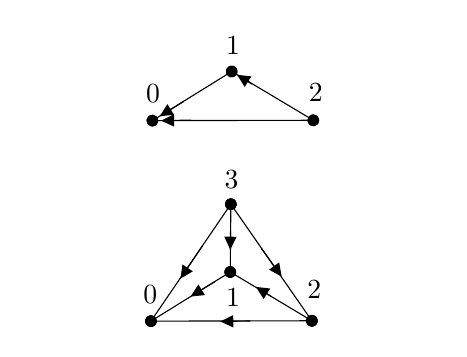
\begin{tikzpicture}[x=0.75pt,y=0.75pt,yscale=-0.7,xscale=0.7]\tikzset{every picture/.style={line width=0.75pt}}

%Straight Lines [id:da31341595090350494] 
\draw    (149.25,245.25) -- (38.5,245.5) ;
\draw [shift={(38.5,245.5)}, rotate = 179.87] [color={rgb, 255:red, 0; green, 0; blue, 0 }  ][fill={rgb, 255:red, 0; green, 0; blue, 0 }  ][line width=0.75]      (0, 0) circle [x radius= 3.35, y radius= 3.35]   ;
\draw [shift={(149.25,245.25)}, rotate = 179.87] [color={rgb, 255:red, 0; green, 0; blue, 0 }  ][fill={rgb, 255:red, 0; green, 0; blue, 0 }  ][line width=0.75]      (0, 0) circle [x radius= 3.35, y radius= 3.35]   ;
%Straight Lines [id:da9609296906616727] 
\draw    (106.88,245.38) -- (88.25,245.71) ;
\draw [shift={(86.25,245.75)}, rotate = 358.96000000000004] [fill={rgb, 255:red, 0; green, 0; blue, 0 }  ][line width=0.75]  [draw opacity=0] (8.93,-4.29) -- (0,0) -- (8.93,4.29) -- cycle    ;

%Straight Lines [id:da252345846123192] 
\draw    (93.5,165) -- (38.5,245.5) ;
\draw [shift={(38.5,245.5)}, rotate = 124.34] [color={rgb, 255:red, 0; green, 0; blue, 0 }  ][fill={rgb, 255:red, 0; green, 0; blue, 0 }  ][line width=0.75]      (0, 0) circle [x radius= 3.35, y radius= 3.35]   ;
\draw [shift={(93.5,165)}, rotate = 124.34] [color={rgb, 255:red, 0; green, 0; blue, 0 }  ][fill={rgb, 255:red, 0; green, 0; blue, 0 }  ][line width=0.75]      (0, 0) circle [x radius= 3.35, y radius= 3.35]   ;
%Straight Lines [id:da11171836378352906] 
\draw    (73.96,193.6) -- (59.88,214.61) ;
\draw [shift={(58.77,216.27)}, rotate = 303.83] [fill={rgb, 255:red, 0; green, 0; blue, 0 }  ][line width=0.75]  [draw opacity=0] (8.93,-4.29) -- (0,0) -- (8.93,4.29) -- cycle    ;

%Straight Lines [id:da9411846809932387] 
\draw    (149.25,245.25) -- (93.5,165) ;
\draw [shift={(93.5,165)}, rotate = 235.21] [color={rgb, 255:red, 0; green, 0; blue, 0 }  ][fill={rgb, 255:red, 0; green, 0; blue, 0 }  ][line width=0.75]      (0, 0) circle [x radius= 3.35, y radius= 3.35]   ;
\draw [shift={(149.25,245.25)}, rotate = 235.21] [color={rgb, 255:red, 0; green, 0; blue, 0 }  ][fill={rgb, 255:red, 0; green, 0; blue, 0 }  ][line width=0.75]      (0, 0) circle [x radius= 3.35, y radius= 3.35]   ;
%Straight Lines [id:da6467035917598132] 
\draw    (114.71,195.71) -- (127.31,213.19) ;
\draw [shift={(128.48,214.81)}, rotate = 234.21] [fill={rgb, 255:red, 0; green, 0; blue, 0 }  ][line width=0.75]  [draw opacity=0] (8.93,-4.29) -- (0,0) -- (8.93,4.29) -- cycle    ;

%Straight Lines [id:da05960945318721844] 
\draw    (93.5,165) -- (93.08,211.67) ;
\draw [shift={(93.08,211.67)}, rotate = 90.51] [color={rgb, 255:red, 0; green, 0; blue, 0 }  ][fill={rgb, 255:red, 0; green, 0; blue, 0 }  ][line width=0.75]      (0, 0) circle [x radius= 3.35, y radius= 3.35]   ;
\draw [shift={(93.5,165)}, rotate = 90.51] [color={rgb, 255:red, 0; green, 0; blue, 0 }  ][fill={rgb, 255:red, 0; green, 0; blue, 0 }  ][line width=0.75]      (0, 0) circle [x radius= 3.35, y radius= 3.35]   ;
%Straight Lines [id:da18779983245814547] 
\draw    (93.08,211.67) -- (38.5,245.5) ;
\draw [shift={(38.5,245.5)}, rotate = 148.21] [color={rgb, 255:red, 0; green, 0; blue, 0 }  ][fill={rgb, 255:red, 0; green, 0; blue, 0 }  ][line width=0.75]      (0, 0) circle [x radius= 3.35, y radius= 3.35]   ;
\draw [shift={(93.08,211.67)}, rotate = 148.21] [color={rgb, 255:red, 0; green, 0; blue, 0 }  ][fill={rgb, 255:red, 0; green, 0; blue, 0 }  ][line width=0.75]      (0, 0) circle [x radius= 3.35, y radius= 3.35]   ;
%Straight Lines [id:da9874513451972009] 
\draw    (93.08,211.67) -- (149.25,245.25) ;
\draw [shift={(149.25,245.25)}, rotate = 30.88] [color={rgb, 255:red, 0; green, 0; blue, 0 }  ][fill={rgb, 255:red, 0; green, 0; blue, 0 }  ][line width=0.75]      (0, 0) circle [x radius= 3.35, y radius= 3.35]   ;
\draw [shift={(93.08,211.67)}, rotate = 30.88] [color={rgb, 255:red, 0; green, 0; blue, 0 }  ][fill={rgb, 255:red, 0; green, 0; blue, 0 }  ][line width=0.75]      (0, 0) circle [x radius= 3.35, y radius= 3.35]   ;
%Straight Lines [id:da21738250880340737] 
\draw    (82.42,218.33) -- (67.49,227.53) ;
\draw [shift={(65.79,228.58)}, rotate = 328.34000000000003] [fill={rgb, 255:red, 0; green, 0; blue, 0 }  ][line width=0.75]  [draw opacity=0] (8.93,-4.29) -- (0,0) -- (8.93,4.29) -- cycle    ;

%Straight Lines [id:da502837847841804] 
\draw    (93.29,183.33) -- (93.13,194.32) ;
\draw [shift={(93.1,196.32)}, rotate = 270.83] [fill={rgb, 255:red, 0; green, 0; blue, 0 }  ][line width=0.75]  [draw opacity=0] (8.93,-4.29) -- (0,0) -- (8.93,4.29) -- cycle    ;

%Straight Lines [id:da38006772268977085] 
\draw    (121.17,228.46) -- (112.46,223) ;
\draw [shift={(110.76,221.94)}, rotate = 392.05] [fill={rgb, 255:red, 0; green, 0; blue, 0 }  ][line width=0.75]  [draw opacity=0] (8.93,-4.29) -- (0,0) -- (8.93,4.29) -- cycle    ;

%Straight Lines [id:da09733860617343582] 
\draw    (150.25,107.25) -- (39.5,107.5) ;
\draw [shift={(39.5,107.5)}, rotate = 179.87] [color={rgb, 255:red, 0; green, 0; blue, 0 }  ][fill={rgb, 255:red, 0; green, 0; blue, 0 }  ][line width=0.75]      (0, 0) circle [x radius= 3.35, y radius= 3.35]   ;
\draw [shift={(150.25,107.25)}, rotate = 179.87] [color={rgb, 255:red, 0; green, 0; blue, 0 }  ][fill={rgb, 255:red, 0; green, 0; blue, 0 }  ][line width=0.75]      (0, 0) circle [x radius= 3.35, y radius= 3.35]   ;
%Straight Lines [id:da9907229664589221] 
\draw    (66.13,107.13) -- (47.5,107.46) ;
\draw [shift={(45.5,107.5)}, rotate = 358.96000000000004] [fill={rgb, 255:red, 0; green, 0; blue, 0 }  ][line width=0.75]  [draw opacity=0] (8.93,-4.29) -- (0,0) -- (8.93,4.29) -- cycle    ;

%Straight Lines [id:da8984506786350759] 
\draw    (94.08,73.67) -- (39.5,107.5) ;
\draw [shift={(39.5,107.5)}, rotate = 148.21] [color={rgb, 255:red, 0; green, 0; blue, 0 }  ][fill={rgb, 255:red, 0; green, 0; blue, 0 }  ][line width=0.75]      (0, 0) circle [x radius= 3.35, y radius= 3.35]   ;
\draw [shift={(94.08,73.67)}, rotate = 148.21] [color={rgb, 255:red, 0; green, 0; blue, 0 }  ][fill={rgb, 255:red, 0; green, 0; blue, 0 }  ][line width=0.75]      (0, 0) circle [x radius= 3.35, y radius= 3.35]   ;
%Straight Lines [id:da13062093153249577] 
\draw    (94.08,73.67) -- (150.25,107.25) ;
\draw [shift={(150.25,107.25)}, rotate = 30.88] [color={rgb, 255:red, 0; green, 0; blue, 0 }  ][fill={rgb, 255:red, 0; green, 0; blue, 0 }  ][line width=0.75]      (0, 0) circle [x radius= 3.35, y radius= 3.35]   ;
\draw [shift={(94.08,73.67)}, rotate = 30.88] [color={rgb, 255:red, 0; green, 0; blue, 0 }  ][fill={rgb, 255:red, 0; green, 0; blue, 0 }  ][line width=0.75]      (0, 0) circle [x radius= 3.35, y radius= 3.35]   ;
%Straight Lines [id:da9384075142317254] 
\draw    (61.13,94.25) -- (46.2,103.45) ;
\draw [shift={(44.5,104.5)}, rotate = 328.34000000000003] [fill={rgb, 255:red, 0; green, 0; blue, 0 }  ][line width=0.75]  [draw opacity=0] (8.93,-4.29) -- (0,0) -- (8.93,4.29) -- cycle    ;

%Straight Lines [id:da2991130569955017] 
\draw    (108.17,82.46) -- (99.46,77) ;
\draw [shift={(97.76,75.94)}, rotate = 392.05] [fill={rgb, 255:red, 0; green, 0; blue, 0 }  ][line width=0.75]  [draw opacity=0] (8.93,-4.29) -- (0,0) -- (8.93,4.29) -- cycle    ;


% Text Node
\draw (94,148) node   {$3$};
% Text Node
\draw (152,88) node   {$2$};
% Text Node
\draw (95,56) node   {$1$};
% Text Node
\draw (151,224) node   {$2$};
% Text Node
\draw (95,229) node   {$1$};
% Text Node
\draw (38,227) node   {$0$};
% Text Node
\draw (40,89) node   {$0$};


\draw (-40,89) node   {};
\draw (230,56) node   {};

\end{tikzpicture}
}}
%			{\centering\\\onslide<2->{ von Neumann ordinals:\\
%					$0=\emptyset$;}
%				\onslide<3->{$1=\bra{\emptyset}$;}
%				\onslide<4->{$2=\bra{\emptyset, \bra{\emptyset}}$;}
%				\onslide<5->{$3=\bra{\emptyset,\bra{\emptyset},\bra{\emptyset,\bra{\emptyset}}}$}}
%		\end{figure}
%\end{frame}}
\showCILC{false}{
	\begin{frame}{\Wf\ sets}
		\begin{block}{\Wf\ set \cite{Aczel1989-ACZNS-2}}
			Let $E$ be a set, $E^\prime$ one of its elements, $E^{\prime\prime}$ any element of $E^\prime$, and so on. A \emphSlide{descent} is the sequence of steps from $E$ to $E^\prime$, $E^\prime$ to $E^{\prime\prime}$, etc.  A set is
			\emphSlide{\wf}\ (or \emphSlide{ordinary}) when it only gives rise to finite descents.
		\end{block}

		\vspace{-0.2cm}
		\begin{figure}
			{\scalebox{0.7}{

\tikzset{every picture/.style={line width=0.75pt}} %set default line width to 0.75pt        

\begin{tikzpicture}[x=0.75pt,y=0.75pt,yscale=-0.7,xscale=0.7]
%uncomment if require: \path (0,243); %set diagram left start at 0, and has height of 243

%Straight Lines [id:da42363008311855377] 
\draw    (126.5,47) ;
\draw [shift={(126.5,47)}, rotate = 0] [color={rgb, 255:red, 0; green, 0; blue, 0 }  ][fill={rgb, 255:red, 0; green, 0; blue, 0 }  ][line width=0.75]      (0, 0) circle [x radius= 3.35, y radius= 3.35]   ;

%Straight Lines [id:da9776475110732991] 
\draw    (196.5,47) -- (196.5,111) ;
\draw [shift={(196.5,111)}, rotate = 90] [color={rgb, 255:red, 0; green, 0; blue, 0 }  ][fill={rgb, 255:red, 0; green, 0; blue, 0 }  ][line width=0.75]      (0, 0) circle [x radius= 3.35, y radius= 3.35]   ;
\draw [shift={(196.5,47)}, rotate = 90] [color={rgb, 255:red, 0; green, 0; blue, 0 }  ][fill={rgb, 255:red, 0; green, 0; blue, 0 }  ][line width=0.75]      (0, 0) circle [x radius= 3.35, y radius= 3.35]   ;
%Straight Lines [id:da161306486001776] 
\draw    (300.5,47) -- (274.5,110) ;
\draw [shift={(274.5,110)}, rotate = 112.43] [color={rgb, 255:red, 0; green, 0; blue, 0 }  ][fill={rgb, 255:red, 0; green, 0; blue, 0 }  ][line width=0.75]      (0, 0) circle [x radius= 3.35, y radius= 3.35]   ;
\draw [shift={(300.5,47)}, rotate = 112.43] [color={rgb, 255:red, 0; green, 0; blue, 0 }  ][fill={rgb, 255:red, 0; green, 0; blue, 0 }  ][line width=0.75]      (0, 0) circle [x radius= 3.35, y radius= 3.35]   ;
%Straight Lines [id:da12831723727076116] 
\draw    (300.5,47) -- (323.5,110) ;
\draw [shift={(323.5,110)}, rotate = 69.94] [color={rgb, 255:red, 0; green, 0; blue, 0 }  ][fill={rgb, 255:red, 0; green, 0; blue, 0 }  ][line width=0.75]      (0, 0) circle [x radius= 3.35, y radius= 3.35]   ;
\draw [shift={(300.5,47)}, rotate = 69.94] [color={rgb, 255:red, 0; green, 0; blue, 0 }  ][fill={rgb, 255:red, 0; green, 0; blue, 0 }  ][line width=0.75]      (0, 0) circle [x radius= 3.35, y radius= 3.35]   ;
%Straight Lines [id:da5112115278285075] 
\draw    (323.5,110) -- (323.5,172) ;
\draw [shift={(323.5,172)}, rotate = 90] [color={rgb, 255:red, 0; green, 0; blue, 0 }  ][fill={rgb, 255:red, 0; green, 0; blue, 0 }  ][line width=0.75]      (0, 0) circle [x radius= 3.35, y radius= 3.35]   ;
\draw [shift={(323.5,110)}, rotate = 90] [color={rgb, 255:red, 0; green, 0; blue, 0 }  ][fill={rgb, 255:red, 0; green, 0; blue, 0 }  ][line width=0.75]      (0, 0) circle [x radius= 3.35, y radius= 3.35]   ;
%Straight Lines [id:da8536132167008245] 
\draw    (426.5,46) -- (400.5,109) ;
\draw [shift={(400.5,109)}, rotate = 112.43] [color={rgb, 255:red, 0; green, 0; blue, 0 }  ][fill={rgb, 255:red, 0; green, 0; blue, 0 }  ][line width=0.75]      (0, 0) circle [x radius= 3.35, y radius= 3.35]   ;
\draw [shift={(426.5,46)}, rotate = 112.43] [color={rgb, 255:red, 0; green, 0; blue, 0 }  ][fill={rgb, 255:red, 0; green, 0; blue, 0 }  ][line width=0.75]      (0, 0) circle [x radius= 3.35, y radius= 3.35]   ;
%Straight Lines [id:da7449065643500326] 
\draw    (426.5,46) -- (449.5,109) ;
\draw [shift={(449.5,109)}, rotate = 69.94] [color={rgb, 255:red, 0; green, 0; blue, 0 }  ][fill={rgb, 255:red, 0; green, 0; blue, 0 }  ][line width=0.75]      (0, 0) circle [x radius= 3.35, y radius= 3.35]   ;
\draw [shift={(426.5,46)}, rotate = 69.94] [color={rgb, 255:red, 0; green, 0; blue, 0 }  ][fill={rgb, 255:red, 0; green, 0; blue, 0 }  ][line width=0.75]      (0, 0) circle [x radius= 3.35, y radius= 3.35]   ;
%Straight Lines [id:da07257306396931185] 
\draw    (449.5,109) -- (449.5,171) ;
\draw [shift={(449.5,171)}, rotate = 90] [color={rgb, 255:red, 0; green, 0; blue, 0 }  ][fill={rgb, 255:red, 0; green, 0; blue, 0 }  ][line width=0.75]      (0, 0) circle [x radius= 3.35, y radius= 3.35]   ;
\draw [shift={(449.5,109)}, rotate = 90] [color={rgb, 255:red, 0; green, 0; blue, 0 }  ][fill={rgb, 255:red, 0; green, 0; blue, 0 }  ][line width=0.75]      (0, 0) circle [x radius= 3.35, y radius= 3.35]   ;
%Straight Lines [id:da021322635576809246] 
\draw    (426.5,46) -- (494.5,110) ;
\draw [shift={(494.5,110)}, rotate = 43.26] [color={rgb, 255:red, 0; green, 0; blue, 0 }  ][fill={rgb, 255:red, 0; green, 0; blue, 0 }  ][line width=0.75]      (0, 0) circle [x radius= 3.35, y radius= 3.35]   ;
\draw [shift={(426.5,46)}, rotate = 43.26] [color={rgb, 255:red, 0; green, 0; blue, 0 }  ][fill={rgb, 255:red, 0; green, 0; blue, 0 }  ][line width=0.75]      (0, 0) circle [x radius= 3.35, y radius= 3.35]   ;
%Straight Lines [id:da9755353003788908] 
\draw    (494.5,110) -- (468.5,173) ;
\draw [shift={(468.5,173)}, rotate = 112.43] [color={rgb, 255:red, 0; green, 0; blue, 0 }  ][fill={rgb, 255:red, 0; green, 0; blue, 0 }  ][line width=0.75]      (0, 0) circle [x radius= 3.35, y radius= 3.35]   ;
\draw [shift={(494.5,110)}, rotate = 112.43] [color={rgb, 255:red, 0; green, 0; blue, 0 }  ][fill={rgb, 255:red, 0; green, 0; blue, 0 }  ][line width=0.75]      (0, 0) circle [x radius= 3.35, y radius= 3.35]   ;
%Straight Lines [id:da12250203413215166] 
\draw    (494.5,110) -- (517.5,173) ;
\draw [shift={(517.5,173)}, rotate = 69.94] [color={rgb, 255:red, 0; green, 0; blue, 0 }  ][fill={rgb, 255:red, 0; green, 0; blue, 0 }  ][line width=0.75]      (0, 0) circle [x radius= 3.35, y radius= 3.35]   ;
\draw [shift={(494.5,110)}, rotate = 69.94] [color={rgb, 255:red, 0; green, 0; blue, 0 }  ][fill={rgb, 255:red, 0; green, 0; blue, 0 }  ][line width=0.75]      (0, 0) circle [x radius= 3.35, y radius= 3.35]   ;
%Straight Lines [id:da4220154805716767] 
\draw    (517.5,173) -- (517.5,235) ;
\draw [shift={(517.5,235)}, rotate = 90] [color={rgb, 255:red, 0; green, 0; blue, 0 }  ][fill={rgb, 255:red, 0; green, 0; blue, 0 }  ][line width=0.75]      (0, 0) circle [x radius= 3.35, y radius= 3.35]   ;
\draw [shift={(517.5,173)}, rotate = 90] [color={rgb, 255:red, 0; green, 0; blue, 0 }  ][fill={rgb, 255:red, 0; green, 0; blue, 0 }  ][line width=0.75]      (0, 0) circle [x radius= 3.35, y radius= 3.35]   ;
%Straight Lines [id:da34828451096237323] 
\draw    (438,77.5) -- (441.87,89.1) ;
\draw [shift={(442.5,91)}, rotate = 251.57] [fill={rgb, 255:red, 0; green, 0; blue, 0 }  ][line width=0.75]  [draw opacity=0] (8.93,-4.29) -- (0,0) -- (8.93,4.29) -- cycle    ;

%Straight Lines [id:da847083601142183] 
\draw    (413.5,77.5) -- (410.21,86.13) ;
\draw [shift={(409.5,88)}, rotate = 290.85] [fill={rgb, 255:red, 0; green, 0; blue, 0 }  ][line width=0.75]  [draw opacity=0] (8.93,-4.29) -- (0,0) -- (8.93,4.29) -- cycle    ;

%Straight Lines [id:da8305126214716252] 
\draw    (449.5,137) -- (449.5,145) ;
\draw [shift={(449.5,147)}, rotate = 270] [fill={rgb, 255:red, 0; green, 0; blue, 0 }  ][line width=0.75]  [draw opacity=0] (8.93,-4.29) -- (0,0) -- (8.93,4.29) -- cycle    ;

%Straight Lines [id:da0020619886975261625] 
\draw    (506,141.5) -- (509.77,151.14) ;
\draw [shift={(510.5,153)}, rotate = 248.63] [fill={rgb, 255:red, 0; green, 0; blue, 0 }  ][line width=0.75]  [draw opacity=0] (8.93,-4.29) -- (0,0) -- (8.93,4.29) -- cycle    ;

%Straight Lines [id:da8008262780720901] 
\draw    (517.5,204) -- (517.5,212) ;
\draw [shift={(517.5,214)}, rotate = 270] [fill={rgb, 255:red, 0; green, 0; blue, 0 }  ][line width=0.75]  [draw opacity=0] (8.93,-4.29) -- (0,0) -- (8.93,4.29) -- cycle    ;

%Straight Lines [id:da5166796275526594] 
\draw    (481.5,141.5) -- (477.3,151.17) ;
\draw [shift={(476.5,153)}, rotate = 293.5] [fill={rgb, 255:red, 0; green, 0; blue, 0 }  ][line width=0.75]  [draw opacity=0] (8.93,-4.29) -- (0,0) -- (8.93,4.29) -- cycle    ;

%Straight Lines [id:da2483045453323448] 
\draw    (460.5,78) -- (472.03,88.64) ;
\draw [shift={(473.5,90)}, rotate = 222.71] [fill={rgb, 255:red, 0; green, 0; blue, 0 }  ][line width=0.75]  [draw opacity=0] (8.93,-4.29) -- (0,0) -- (8.93,4.29) -- cycle    ;


%Straight Lines [id:da5301987015108148] 
\draw    (196.5,69) -- (196.5,77) ;
\draw [shift={(196.5,79)}, rotate = 270] [fill={rgb, 255:red, 0; green, 0; blue, 0 }  ][line width=0.75]  [draw opacity=0] (8.93,-4.29) -- (0,0) -- (8.93,4.29) -- cycle    ;

%Straight Lines [id:da9808201842892292] 
\draw    (287.5,78.5) -- (282.22,92.13) ;
\draw [shift={(281.5,94)}, rotate = 291.15999999999997] [fill={rgb, 255:red, 0; green, 0; blue, 0 }  ][line width=0.75]  [draw opacity=0] (8.93,-4.29) -- (0,0) -- (8.93,4.29) -- cycle    ;

%Straight Lines [id:da9287523922345057] 
\draw    (313,82.5) -- (316.82,93.12) ;
\draw [shift={(317.5,95)}, rotate = 250.2] [fill={rgb, 255:red, 0; green, 0; blue, 0 }  ][line width=0.75]  [draw opacity=0] (8.93,-4.29) -- (0,0) -- (8.93,4.29) -- cycle    ;

%Straight Lines [id:da02578212493217935] 
\draw    (323.5,141) -- (323.5,149) ;
\draw [shift={(323.5,151)}, rotate = 270] [fill={rgb, 255:red, 0; green, 0; blue, 0 }  ][line width=0.75]  [draw opacity=0] (8.93,-4.29) -- (0,0) -- (8.93,4.29) -- cycle    ;


% Text Node
\draw (130,22) node   {$0$};
% Text Node
\draw (197,22) node   {$1$};
% Text Node
\draw (300,22) node   {$2$};
% Text Node
\draw (427,22) node   {$3$};


\draw (60,22) node   {};
\draw (585,22) node   {};


\end{tikzpicture}

}\label{subfig-1:von_neu_ord}}
			\hfill
			{\scalebox{1}{\tikzset{every picture/.style={line width=0.75pt}} %set default line width to 0.75pt        

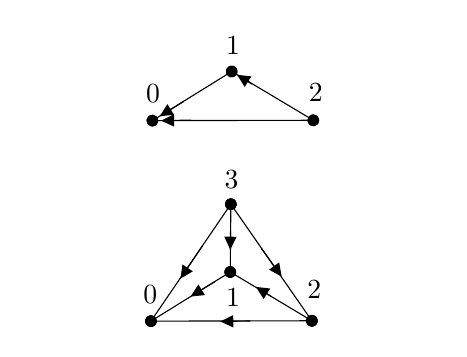
\begin{tikzpicture}[x=0.75pt,y=0.75pt,yscale=-0.7,xscale=0.7]\tikzset{every picture/.style={line width=0.75pt}}

%Straight Lines [id:da31341595090350494] 
\draw    (149.25,245.25) -- (38.5,245.5) ;
\draw [shift={(38.5,245.5)}, rotate = 179.87] [color={rgb, 255:red, 0; green, 0; blue, 0 }  ][fill={rgb, 255:red, 0; green, 0; blue, 0 }  ][line width=0.75]      (0, 0) circle [x radius= 3.35, y radius= 3.35]   ;
\draw [shift={(149.25,245.25)}, rotate = 179.87] [color={rgb, 255:red, 0; green, 0; blue, 0 }  ][fill={rgb, 255:red, 0; green, 0; blue, 0 }  ][line width=0.75]      (0, 0) circle [x radius= 3.35, y radius= 3.35]   ;
%Straight Lines [id:da9609296906616727] 
\draw    (106.88,245.38) -- (88.25,245.71) ;
\draw [shift={(86.25,245.75)}, rotate = 358.96000000000004] [fill={rgb, 255:red, 0; green, 0; blue, 0 }  ][line width=0.75]  [draw opacity=0] (8.93,-4.29) -- (0,0) -- (8.93,4.29) -- cycle    ;

%Straight Lines [id:da252345846123192] 
\draw    (93.5,165) -- (38.5,245.5) ;
\draw [shift={(38.5,245.5)}, rotate = 124.34] [color={rgb, 255:red, 0; green, 0; blue, 0 }  ][fill={rgb, 255:red, 0; green, 0; blue, 0 }  ][line width=0.75]      (0, 0) circle [x radius= 3.35, y radius= 3.35]   ;
\draw [shift={(93.5,165)}, rotate = 124.34] [color={rgb, 255:red, 0; green, 0; blue, 0 }  ][fill={rgb, 255:red, 0; green, 0; blue, 0 }  ][line width=0.75]      (0, 0) circle [x radius= 3.35, y radius= 3.35]   ;
%Straight Lines [id:da11171836378352906] 
\draw    (73.96,193.6) -- (59.88,214.61) ;
\draw [shift={(58.77,216.27)}, rotate = 303.83] [fill={rgb, 255:red, 0; green, 0; blue, 0 }  ][line width=0.75]  [draw opacity=0] (8.93,-4.29) -- (0,0) -- (8.93,4.29) -- cycle    ;

%Straight Lines [id:da9411846809932387] 
\draw    (149.25,245.25) -- (93.5,165) ;
\draw [shift={(93.5,165)}, rotate = 235.21] [color={rgb, 255:red, 0; green, 0; blue, 0 }  ][fill={rgb, 255:red, 0; green, 0; blue, 0 }  ][line width=0.75]      (0, 0) circle [x radius= 3.35, y radius= 3.35]   ;
\draw [shift={(149.25,245.25)}, rotate = 235.21] [color={rgb, 255:red, 0; green, 0; blue, 0 }  ][fill={rgb, 255:red, 0; green, 0; blue, 0 }  ][line width=0.75]      (0, 0) circle [x radius= 3.35, y radius= 3.35]   ;
%Straight Lines [id:da6467035917598132] 
\draw    (114.71,195.71) -- (127.31,213.19) ;
\draw [shift={(128.48,214.81)}, rotate = 234.21] [fill={rgb, 255:red, 0; green, 0; blue, 0 }  ][line width=0.75]  [draw opacity=0] (8.93,-4.29) -- (0,0) -- (8.93,4.29) -- cycle    ;

%Straight Lines [id:da05960945318721844] 
\draw    (93.5,165) -- (93.08,211.67) ;
\draw [shift={(93.08,211.67)}, rotate = 90.51] [color={rgb, 255:red, 0; green, 0; blue, 0 }  ][fill={rgb, 255:red, 0; green, 0; blue, 0 }  ][line width=0.75]      (0, 0) circle [x radius= 3.35, y radius= 3.35]   ;
\draw [shift={(93.5,165)}, rotate = 90.51] [color={rgb, 255:red, 0; green, 0; blue, 0 }  ][fill={rgb, 255:red, 0; green, 0; blue, 0 }  ][line width=0.75]      (0, 0) circle [x radius= 3.35, y radius= 3.35]   ;
%Straight Lines [id:da18779983245814547] 
\draw    (93.08,211.67) -- (38.5,245.5) ;
\draw [shift={(38.5,245.5)}, rotate = 148.21] [color={rgb, 255:red, 0; green, 0; blue, 0 }  ][fill={rgb, 255:red, 0; green, 0; blue, 0 }  ][line width=0.75]      (0, 0) circle [x radius= 3.35, y radius= 3.35]   ;
\draw [shift={(93.08,211.67)}, rotate = 148.21] [color={rgb, 255:red, 0; green, 0; blue, 0 }  ][fill={rgb, 255:red, 0; green, 0; blue, 0 }  ][line width=0.75]      (0, 0) circle [x radius= 3.35, y radius= 3.35]   ;
%Straight Lines [id:da9874513451972009] 
\draw    (93.08,211.67) -- (149.25,245.25) ;
\draw [shift={(149.25,245.25)}, rotate = 30.88] [color={rgb, 255:red, 0; green, 0; blue, 0 }  ][fill={rgb, 255:red, 0; green, 0; blue, 0 }  ][line width=0.75]      (0, 0) circle [x radius= 3.35, y radius= 3.35]   ;
\draw [shift={(93.08,211.67)}, rotate = 30.88] [color={rgb, 255:red, 0; green, 0; blue, 0 }  ][fill={rgb, 255:red, 0; green, 0; blue, 0 }  ][line width=0.75]      (0, 0) circle [x radius= 3.35, y radius= 3.35]   ;
%Straight Lines [id:da21738250880340737] 
\draw    (82.42,218.33) -- (67.49,227.53) ;
\draw [shift={(65.79,228.58)}, rotate = 328.34000000000003] [fill={rgb, 255:red, 0; green, 0; blue, 0 }  ][line width=0.75]  [draw opacity=0] (8.93,-4.29) -- (0,0) -- (8.93,4.29) -- cycle    ;

%Straight Lines [id:da502837847841804] 
\draw    (93.29,183.33) -- (93.13,194.32) ;
\draw [shift={(93.1,196.32)}, rotate = 270.83] [fill={rgb, 255:red, 0; green, 0; blue, 0 }  ][line width=0.75]  [draw opacity=0] (8.93,-4.29) -- (0,0) -- (8.93,4.29) -- cycle    ;

%Straight Lines [id:da38006772268977085] 
\draw    (121.17,228.46) -- (112.46,223) ;
\draw [shift={(110.76,221.94)}, rotate = 392.05] [fill={rgb, 255:red, 0; green, 0; blue, 0 }  ][line width=0.75]  [draw opacity=0] (8.93,-4.29) -- (0,0) -- (8.93,4.29) -- cycle    ;

%Straight Lines [id:da09733860617343582] 
\draw    (150.25,107.25) -- (39.5,107.5) ;
\draw [shift={(39.5,107.5)}, rotate = 179.87] [color={rgb, 255:red, 0; green, 0; blue, 0 }  ][fill={rgb, 255:red, 0; green, 0; blue, 0 }  ][line width=0.75]      (0, 0) circle [x radius= 3.35, y radius= 3.35]   ;
\draw [shift={(150.25,107.25)}, rotate = 179.87] [color={rgb, 255:red, 0; green, 0; blue, 0 }  ][fill={rgb, 255:red, 0; green, 0; blue, 0 }  ][line width=0.75]      (0, 0) circle [x radius= 3.35, y radius= 3.35]   ;
%Straight Lines [id:da9907229664589221] 
\draw    (66.13,107.13) -- (47.5,107.46) ;
\draw [shift={(45.5,107.5)}, rotate = 358.96000000000004] [fill={rgb, 255:red, 0; green, 0; blue, 0 }  ][line width=0.75]  [draw opacity=0] (8.93,-4.29) -- (0,0) -- (8.93,4.29) -- cycle    ;

%Straight Lines [id:da8984506786350759] 
\draw    (94.08,73.67) -- (39.5,107.5) ;
\draw [shift={(39.5,107.5)}, rotate = 148.21] [color={rgb, 255:red, 0; green, 0; blue, 0 }  ][fill={rgb, 255:red, 0; green, 0; blue, 0 }  ][line width=0.75]      (0, 0) circle [x radius= 3.35, y radius= 3.35]   ;
\draw [shift={(94.08,73.67)}, rotate = 148.21] [color={rgb, 255:red, 0; green, 0; blue, 0 }  ][fill={rgb, 255:red, 0; green, 0; blue, 0 }  ][line width=0.75]      (0, 0) circle [x radius= 3.35, y radius= 3.35]   ;
%Straight Lines [id:da13062093153249577] 
\draw    (94.08,73.67) -- (150.25,107.25) ;
\draw [shift={(150.25,107.25)}, rotate = 30.88] [color={rgb, 255:red, 0; green, 0; blue, 0 }  ][fill={rgb, 255:red, 0; green, 0; blue, 0 }  ][line width=0.75]      (0, 0) circle [x radius= 3.35, y radius= 3.35]   ;
\draw [shift={(94.08,73.67)}, rotate = 30.88] [color={rgb, 255:red, 0; green, 0; blue, 0 }  ][fill={rgb, 255:red, 0; green, 0; blue, 0 }  ][line width=0.75]      (0, 0) circle [x radius= 3.35, y radius= 3.35]   ;
%Straight Lines [id:da9384075142317254] 
\draw    (61.13,94.25) -- (46.2,103.45) ;
\draw [shift={(44.5,104.5)}, rotate = 328.34000000000003] [fill={rgb, 255:red, 0; green, 0; blue, 0 }  ][line width=0.75]  [draw opacity=0] (8.93,-4.29) -- (0,0) -- (8.93,4.29) -- cycle    ;

%Straight Lines [id:da2991130569955017] 
\draw    (108.17,82.46) -- (99.46,77) ;
\draw [shift={(97.76,75.94)}, rotate = 392.05] [fill={rgb, 255:red, 0; green, 0; blue, 0 }  ][line width=0.75]  [draw opacity=0] (8.93,-4.29) -- (0,0) -- (8.93,4.29) -- cycle    ;


% Text Node
\draw (94,148) node   {$3$};
% Text Node
\draw (152,88) node   {$2$};
% Text Node
\draw (95,56) node   {$1$};
% Text Node
\draw (151,224) node   {$2$};
% Text Node
\draw (95,229) node   {$1$};
% Text Node
\draw (38,227) node   {$0$};
% Text Node
\draw (40,89) node   {$0$};


\draw (-40,89) node   {};
\draw (230,56) node   {};

\end{tikzpicture}
}}
		\end{figure}
		\centering von Neumann ordinals:\\
		$0=\emptyset$;
		$1=\bra{\emptyset}$;
		$2=\bra{\emptyset, \bra{\emptyset}}$;
		$3=\bra{\emptyset,\bra{\emptyset},\bra{\emptyset,\bra{\emptyset}}}$
	\end{frame}
}

\showCILC{true}{
	\begin{frame}{\Nwf\ sets}
		\begin{block}{\Nwf\ set~\cite{Aczel1989-ACZNS-2}}
			A set is \emphSlide{\nwf}\ (or \emphSlide{extraordinary}) when among its descents there are some which are infinite.
		\end{block}
		\centering
		\begin{figure}
			{\scalebox{0.6}{\input{img/omega}}}
			\hfill
			{\scalebox{1.2}{

\tikzset{every picture/.style={line width=0.75pt}} %set default line width to 0.75pt        

\begin{tikzpicture}[x=0.75pt,y=0.75pt,yscale=-1,xscale=1]
%uncomment if require: \path (0,300); %set diagram left start at 0, and has height of 300

%Straight Lines [id:da6276790682079358] 
\draw    (100.6,110) -- (140.85,110) ;


%Flowchart: Connector [id:dp10712755168097865] 
\draw  [fill={rgb, 255:red, 0; green, 0; blue, 0 }  ,fill opacity=1 ] (103,110) .. controls (103,111.33) and (101.93,112.4) .. (100.6,112.4) .. controls (99.27,112.4) and (98.2,111.33) .. (98.2,110) .. controls (98.2,108.67) and (99.27,107.6) .. (100.6,107.6) .. controls (101.93,107.6) and (103,108.67) .. (103,110) -- cycle ;
%Straight Lines [id:da8191358904406301] 
\draw    (139.8,110.2) -- (180.05,110.2) ;


%Flowchart: Connector [id:dp9628511983929124] 
\draw  [fill={rgb, 255:red, 0; green, 0; blue, 0 }  ,fill opacity=1 ] (142.2,110.2) .. controls (142.2,111.53) and (141.13,112.6) .. (139.8,112.6) .. controls (138.47,112.6) and (137.4,111.53) .. (137.4,110.2) .. controls (137.4,108.87) and (138.47,107.8) .. (139.8,107.8) .. controls (141.13,107.8) and (142.2,108.87) .. (142.2,110.2) -- cycle ;
%Shape: Triangle [id:dp18185199166706778] 
\draw  [fill={rgb, 255:red, 0; green, 0; blue, 0 }  ,fill opacity=1 ] (120.72,110) -- (118,111.21) -- (118,108.79) -- cycle ;
%Shape: Triangle [id:dp11767706980455106] 
\draw  [color={rgb, 255:red, 0; green, 0; blue, 0 }  ,draw opacity=1 ][fill={rgb, 255:red, 0; green, 0; blue, 0 }  ,fill opacity=1 ] (159.92,110.2) -- (157.2,111.41) -- (157.2,108.99) -- cycle ;
%Straight Lines [id:da6334935852876922] 
\draw    (180.1,110) -- (220.35,110) ;


%Flowchart: Connector [id:dp022374442404981654] 
\draw  [fill={rgb, 255:red, 0; green, 0; blue, 0 }  ,fill opacity=1 ] (182.5,110) .. controls (182.5,111.33) and (181.43,112.4) .. (180.1,112.4) .. controls (178.77,112.4) and (177.7,111.33) .. (177.7,110) .. controls (177.7,108.67) and (178.77,107.6) .. (180.1,107.6) .. controls (181.43,107.6) and (182.5,108.67) .. (182.5,110) -- cycle ;
%Flowchart: Connector [id:dp8113410302855639] 
\draw  [fill={rgb, 255:red, 0; green, 0; blue, 0 }  ,fill opacity=1 ] (221.7,110.2) .. controls (221.7,111.53) and (220.63,112.6) .. (219.3,112.6) .. controls (217.97,112.6) and (216.9,111.53) .. (216.9,110.2) .. controls (216.9,108.87) and (217.97,107.8) .. (219.3,107.8) .. controls (220.63,107.8) and (221.7,108.87) .. (221.7,110.2) -- cycle ;
%Shape: Triangle [id:dp5972516863295354] 
\draw  [fill={rgb, 255:red, 0; green, 0; blue, 0 }  ,fill opacity=1 ] (200.22,110) -- (197.5,111.21) -- (197.5,108.79) -- cycle ;
%Straight Lines [id:da9015443131541547] 
\draw  [dash pattern={on 0.84pt off 2.51pt}]  (219.3,110.2) -- (250.15,110.2) ;

\draw (250,140) node   {};
\draw (90,140) node   {};


\end{tikzpicture}

}}
			\\
			The \nwf\ set $\Omega = \{\Omega\}$
		\end{figure}
	\end{frame}
}

\showCILC{false}{
	\begin{frame}{Consequences}

		\begin{columns}[T] % align columns
			\begin{column}{.48\textwidth}
				{\color{black}\rule{\linewidth}{4pt}
					\Wf\ set Theory}
				\begin{center}
					\emph{Only \wf\ graphs have decorations \textbf{(FA)}\tikzmark{conseqa}}\\
					$\mathbf{\downarrow}$\\
					\emph{Each \wf\ graph is a picture of exactly one set\tikzmark{conseqc}}
				\end{center}

			\end{column}%
			\hfill%
			\onslide<2->{\begin{column}{.48\textwidth}
					{\emphColorSlide{\rule{\linewidth}{4pt}
							\Nwf\ set Theory}}
					\begin{center}
						{\color{ForestGreen!80!white}\emph{Every graph has a decoration \tikzmark{conseqb}\textbf{(AFA)}}\\
							\textbf{$\downarrow$}\\
							\emph{Every graph is a picture of \tikzmark{conseqd}exactly one set}}
					\end{center}
				\end{column}}%
		\end{columns}
		\onslide<2->{
\begin{tikzpicture}[overlay,remember picture]
				\draw[very thick, -Stealth, ForestGreen] ($({pic cs:conseqc})+(1.5ex,9.5ex)$) to ($({pic cs:conseqd})+(-6ex,9.5ex)$);
				\draw[very thick, -Stealth, ForestGreen] ($({pic cs:conseqc})+(1.5ex,1.5ex)$) to ($({pic cs:conseqd})+(-6ex,1.5ex)$);
			\end{tikzpicture}
		}

	\end{frame}
}
\subsection*{}
%	\showCILC{true}{\begin{frame}{From \PosS\ to Kripke Structures}
%		A \nwf\ set can be expressed as a \emph{system of equations}
%		\begin{center}
%			\begin{figure}
%			{\scalebox{0.6}{

\tikzset{every picture/.style={line width=0.75pt}} %set default line width to 0.75pt        

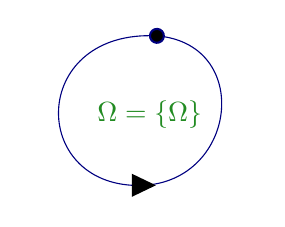
\begin{tikzpicture}[x=0.75pt,y=0.75pt,yscale=-1,xscale=1]
%uncomment if require: \path (0,243); %set diagram left start at 0, and has height of 243

%Curve Lines [id:da9361500626799328] 
\draw [NavyBlue]   (103.5,82) .. controls (151.5,86) and (141.5,157) .. (91.5,154) .. controls (41.5,151) and (43.5,79) .. (103.5,82) -- cycle ;
\draw [shift={(103.5,82)}, rotate = 2.86] [color=NavyBlue][fill={rgb, 255:red, 0; green, 0; blue, 0 }  ][line width=0.75]      (0, 0) circle [x radius= 3.35, y radius= 3.35]   ;

%Straight Lines [id:da3323560662413527] 
\draw [line width=1.5]    (103,154) ;
\draw [shift={(103,154)}, rotate = 180, color=NavyBlue] [fill={rgb, 255:red, 0; green, 0; blue, 0 }  ][line width=1.5]  [draw opacity=0] (11.61,-5.58) -- (0,0) -- (11.61,5.58) -- cycle    ;
\draw[color=ForestGreen] (100,120) node   {$\Omega=\{\Omega\}$};


\end{tikzpicture}

}}
%			\end{figure}
%		\end{center}
%		\vspace{-0.5cm}
%		\begin{center}
%			\textbf{Graphs} and \textbf{system of equations} are representation for \nwf\ set.\\
%			\vspace{0.2cm}
%			\onslide<2->{
%			Each graph has a \emph{unique decoration}}
%			\onslide<3->{
%			\\$\downarrow$\\
%			Each system of equations has a \emph{unique solution}, and  this solution represents a \emph{decoration} for a labelled graph (Kripke structure)  
%			}
%			\onslide<4->{\\$\downarrow$\\
%			\emphSlide{\textbf{A \pos\ correspond with a whole class of bisimilar, but structurally different, Kripke structures}}}
%		\end{center}
%	\end{frame}}

\showCILC{true}{
	\begin{frame}{Formal Definition}
		\begin{block}{\Pos~\cite{Gerbrandy1997}}
			Let \sAG\ be a set of agents and \sP\ a set of propositional variables:
			\begin{itemize}
				\item[-] A \emphSlide{\pos}\ $\poss{u}$ is a function that assigns to each propositional variable $\defemph{\ttSlide{l}} \in \sP$ a truth value $\possarg{u}{\defemph{\ttSlide{l}}} \in \bra{0,1}$ and to each agent $\agentSlide{ag} \in \sAG$ a set of \posS\  $\possarg{u}{\agentSlide{ag}} = \sigma$.
			\end{itemize}
		\end{block}
		\onslide<2>{Intuitively ...
			\begin{itemize}
				\item[-] The \pos\ \poss{u} is a possible interpretation of the world and of the agents' beliefs
				\item[-] $\possarg{u}{\defemph{\ttSlide{l}}}$ specifies the truth value of the literal \defemph{\ttSlide{l}}
				\item[-] $\possarg{u}{\agentSlide{ag}}$ is the set of all the interpretations the agent \agentSlide{ag} considers possible in \poss{u}
			\end{itemize}
		}
	\end{frame}
}


\showCILC{true}{
	\begin{frame}{From \PosS\ to Kripke Structures}
		\tikzmark{froma}Considering a \tikzmark{fromg}\pos\tikzmark{fromf}\\
		\onslide<2->{\hspace*{0.8cm}\tikzmark{fromb}Can be expressed as a \emph{system of equations}\\}
		\onslide<3->{\hspace*{1.6cm}\tikzmark{fromc}Systems of equations have unique solutions\\}
		\onslide<4->{\hspace*{2.4cm}\tikzmark{fromd}The solution decorates a \tikzmark{fromh}Kripke structure\tikzmark{frome}}
		\vfill
		\vspace*{0.6cm}
		\begin{columns}[T] % align columns
			\begin{column}{.2\textwidth}
				{\only<5>{\color{ForestGreen}}
					{\only<5>{\color{ForestGreen}}\rule{\linewidth}{1pt}
						\footnotesize A \pos}
					%\vspace*{0.8cm}%
					\begin{center}
						\hspace*{-0.5cm}%
						{\scalebox{0.5}{\input{img/possibility_p}}}
					\end{center}}
			\end{column}%
			\hfill%
			\onslide<2->{\begin{column}{.35\textwidth}
					{\rule{\linewidth}{1pt}
						\footnotesize Its system of equation}
					\begin{center}
						%\hspace*{-0.6cm}%
						{\scriptsize $\begin{cases}
									\poss{w}(\textcolor{NavyBlue}{p}) = 1    & \poss{w}(\textcolor{NavyBlue}{q}) = 0    \\
									\poss{v}(\textcolor{NavyBlue}{p}) = 1    & \poss{v}(\textcolor{NavyBlue}{q}) = 1    \\
									\poss{u}(\textcolor{NavyBlue}{p}) = 0    & \poss{u}(\textcolor{NavyBlue}{q}) = 0    \\
									\poss{w}(\agentSlide{A}) = \{\poss{v}\}  & \poss{w}(\agentSlide{B}) = \{\emptyset\} \\
									\poss{v}(\agentSlide{A}) = \{\poss{v}\}  & \poss{v}(\agentSlide{B}) = \{\poss{u}\}  \\
									\poss{u}(\agentSlide{A}) = \{\emptyset\} & \poss{u}(\agentSlide{B}) = \{\emptyset\} \\
								\end{cases}$
						}
					\end{center}
				\end{column}}%
			\hfill%
			\onslide<3->{\begin{column}{.2\textwidth}
					{\rule{\linewidth}{1pt}
						\footnotesize The solution}
					\begin{center}
						\hspace{-0.4cm}{\scalebox{0.5}{

\tikzset{every picture/.style={line width=0.75pt}} %set default line width to 0.75pt        

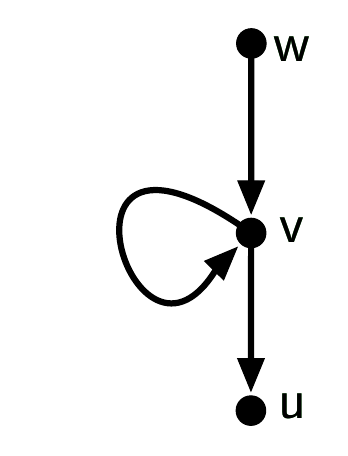
\begin{tikzpicture}[x=0.75pt,y=0.75pt,yscale=-1,xscale=1, opacity=1, fill opacity=1]
%uncomment if require: \path (0,300); %set diagram left start at 0, and has height of 300


%Straight Lines [id:da4670850942943552] 
\draw [line width=2.25]    (231.25,52.67) -- (231.16,126.71) ;
%Curve Lines [id:da34427195808621325] 
\draw [line width=2.25]    (231.14,144) .. controls (124.98,68.18) and (174.97,230.32) .. (215.38,159.61) ;
%Straight Lines [id:da7340515842576736] 
\draw [line width=2.25]    (231.15,138.24) -- (231.06,212.28) ;



%Shape: Triangle [id:dp5511387235098089] 
\draw  [color={rgb, 255:red, 0; green, 0; blue, 0 }][fill={rgb, 255:red, 0; green, 0; blue, 0 }] (231.05,220.06) -- (224.68,204.5) -- (237.45,204.51) -- cycle ;
%Shape: Triangle [id:dp72110595964638] 
\draw  [color={rgb, 255:red, 0; green, 0; blue, 0 }][fill={rgb, 255:red, 0; green, 0; blue, 0 }] (224.33,151.03) -- (217.88,166.55) -- (208.83,157.55) -- cycle ;
%Shape: Triangle [id:dp1921776052623907] 
\draw  [color={rgb, 255:red, 0; green, 0; blue, 0 }][fill={rgb, 255:red, 0; green, 0; blue, 0 }] (231.15,134.49) -- (224.79,118.93) -- (237.55,118.95) -- cycle ;

%Shape: Ellipse [id:dp7930732829426068] 
\draw  [fill={rgb, 255:red, 0; green, 0; blue, 0 }] (231.04,222.47) .. controls (234.97,222.47) and (238.14,225.66) .. (238.14,229.58) .. controls (238.13,233.5) and (234.95,236.68) .. (231.03,236.67) .. controls (227.1,236.67) and (223.93,233.48) .. (223.93,229.56) .. controls (223.94,225.64) and (227.12,222.46) .. (231.04,222.47) -- cycle ;
%Shape: Ellipse [id:dp06243918702040174] 
\draw  [fill={rgb, 255:red, 0; green, 0; blue, 0 }] (231.26,45.57) .. controls (235.18,45.57) and (238.36,48.76) .. (238.35,52.68) .. controls (238.35,56.6) and (235.17,59.78) .. (231.24,59.78) .. controls (227.32,59.77) and (224.14,56.59) .. (224.15,52.66) .. controls (224.15,48.74) and (227.34,45.56) .. (231.26,45.57) -- cycle ;
%Shape: Ellipse [id:dp44126371965490274] 
\draw  [fill={rgb, 255:red, 0; green, 0; blue, 0 }] (231.15,136.9) .. controls (235.07,136.9) and (238.25,140.09) .. (238.24,144.01) .. controls (238.24,147.93) and (235.05,151.11) .. (231.13,151.1) .. controls (227.21,151.1) and (224.03,147.92) .. (224.04,143.99) .. controls (224.04,140.07) and (227.22,136.89) .. (231.15,136.9) -- cycle ;


% Text Node
\onslide<3->{\draw (250.89,55.47) node  [align=left, opacity = 1, ForestGreen] {\huge \poss{w}};
% Text Node
\draw (250.89,142.47) node  [align=left, opacity = 1, ForestGreen] {\huge \poss{v}};
% Text Node
\draw (250.89,227.47) node  [align=left, opacity = 1, ForestGreen] {\huge \poss{u}};
}

% Text Node
\onslide<4->{\draw (250.89,55.47) node  [align=left] {\huge \poss{w}};
% Text Node
\draw (250.89,142.47) node  [align=left] {\huge \poss{v}};
% Text Node
\draw (250.89,227.47) node  [align=left] {\huge \poss{u}};
}

\end{tikzpicture}}}
					\end{center}
				\end{column}}%
			\hfill%
			\onslide<4->{\begin{column}{.35\textwidth}
					{\only<5>{\color{ForestGreen}}
						{\rule{\linewidth}{1pt}
							\footnotesize Relative Kripke Structure}
						\begin{center}
							{\scalebox{0.6}{

\tikzset{every picture/.style={line width=0.75pt}} %set default line width to 0.75pt        

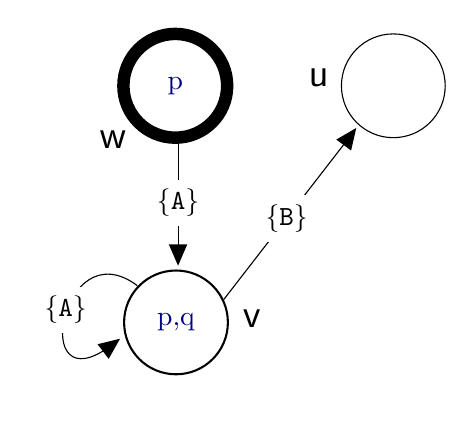
\begin{tikzpicture}[x=0.75pt,y=0.75pt,yscale=-1,xscale=1]
%uncomment if require: \path (0,300); %set diagram left start at 0, and has height of 300

%Straight Lines [id:da7382395640533164] 
\draw    (130.29,59) -- (130.29,118) ;
%Straight Lines [id:da018251469869151382] 
\draw    (152.29,135) -- (213,56.6) ;


%Shape: Circle [id:dp8938158972072578] 
\draw  [line width=0.75]  (104.29,146) .. controls (104.29,132.19) and (115.48,121) .. (129.29,121) .. controls (143.09,121) and (154.29,132.19) .. (154.29,146) .. controls (154.29,159.81) and (143.09,171) .. (129.29,171) .. controls (115.48,171) and (104.29,159.81) .. (104.29,146) -- cycle ;
%Shape: Circle [id:dp19780391712041556] 
\draw   (209,32) .. controls (209,18.19) and (220.19,7) .. (234,7) .. controls (247.81,7) and (259,18.19) .. (259,32) .. controls (259,45.81) and (247.81,57) .. (234,57) .. controls (220.19,57) and (209,45.81) .. (209,32) -- cycle ;
%Shape: Circle [id:dp06782137726568571] 
\draw  [line width=4.5]  (103.95,32) .. controls (103.95,18.19) and (115.15,7) .. (128.95,7) .. controls (142.76,7) and (153.95,18.19) .. (153.95,32) .. controls (153.95,45.81) and (142.76,57) .. (128.95,57) .. controls (115.15,57) and (103.95,45.81) .. (103.95,32) -- cycle ;
%Curve Lines [id:da0862450190271058] 
\draw    (110.62,128.27) .. controls (73.82,100.67) and (58.1,187.08) .. (98.1,157.08) ;

%Shape: Triangle [id:dp4725710951486233] 
\draw  [fill={rgb, 255:red, 0; green, 0; blue, 0 }  ,fill opacity=1 ] (101.8,154.28) -- (96.82,163.08) -- (91.97,156.67) -- cycle ;
%Shape: Triangle [id:dp08394946096129607] 
\draw  [fill={rgb, 255:red, 0; green, 0; blue, 0 }  ,fill opacity=1 ] (215.75,52.87) -- (213.48,62.72) -- (207.01,57.95) -- cycle ;

%Shape: Triangle [id:dp417855807516911] 
\draw  [fill={rgb, 255:red, 0; green, 0; blue, 0 }  ,fill opacity=1 ] (130.29,118) -- (126.27,108.72) -- (134.3,108.72) -- cycle ;


% Text Node
\draw (129.29,146) node  [align=left, NavyBlue] {p,q};
% Text Node
\draw (128.95,32) node  [align=left, NavyBlue] {p};
% Text Node
\draw  [color={rgb, 255:red, 255; green, 255; blue, 255 }  ,draw opacity=1 ][fill={rgb, 255:red, 255; green, 255; blue, 255 }  ,fill opacity=1 ]  (173.64,84.8) -- (191.64,84.8) -- (191.64,106.8) -- (173.64,106.8) -- cycle  ;
\draw (182.64,95.8) node  [align=left] {\{\agentSlide{B}\}};
% Text Node
\draw  [color={rgb, 255:red, 255; green, 255; blue, 255 }  ,draw opacity=1 ][fill={rgb, 255:red, 255; green, 255; blue, 255 }  ,fill opacity=1 ]  (67.14,129) -- (85.14,129) -- (85.14,151) -- (67.14,151) -- cycle  ;
\draw (76.14,140) node  [align=left] {\{\agentSlide{A}\}};
% Text Node
\draw  [color={rgb, 255:red, 255; green, 255; blue, 255 }  ,draw opacity=1 ][fill={rgb, 255:red, 255; green, 255; blue, 255 }  ,fill opacity=1 ]  (121.29,77.5) -- (139.29,77.5) -- (139.29,99.5) -- (121.29,99.5) -- cycle  ;
\draw (130.29,88.5) node  [align=left] {\{\agentSlide{A}\}};
% Text Node
\draw (99,58) node  [align=left] {\Large \poss{w}};
% Text Node
\draw (166,144) node  [align=left] {\Large \poss{v}};
% Text Node
\draw (198,28) node  [align=left] {\Large \poss{u}};


\end{tikzpicture}
}}
						\end{center}
					}
				\end{column}}%
		\end{columns}

		
\begin{tikzpicture}[overlay, remember picture]
			\only<2>{\draw[thick, -Stealth,out=180,in=180,looseness=2, ForestGreen] ($({pic cs:froma})+(-1.5ex,0.5ex)$) to ($({pic cs:fromb})+(-1ex,1.1ex)$);}
			\onslide<3->{\draw[thick, -Stealth,out=180,in=180,looseness=2] ($({pic cs:froma})+(-1.5ex,0.5ex)$) to ($({pic cs:fromb})+(-1ex,1.1ex)$);}
			\only<3>{\draw[thick, -Stealth,out=180,in=180,looseness=2, ForestGreen] ($({pic cs:fromb})+(-1.5ex,0.5ex)$) to ($({pic cs:fromc})+(-1ex,1.1ex)$);}
			\onslide<4->{\draw[thick, -Stealth,out=180,in=180,looseness=2] ($({pic cs:fromb})+(-1.5ex,0.5ex)$) to ($({pic cs:fromc})+(-1ex,1.1ex)$);}
			\only<4>{\draw[thick, -Stealth,out=180,in=180,looseness=2, ForestGreen] ($({pic cs:fromc})+(-1.5ex,0.5ex)$) to ($({pic cs:fromd})+(-1ex,1.1ex)$);}
			\onslide<5->{\draw[thick, -Stealth,out=180,in=180,looseness=2] ($({pic cs:fromc})+(-1.5ex,0.5ex)$) to ($({pic cs:fromd})+(-1ex,1.1ex)$);
				\draw[thick, Stealth-Stealth,out=0,in=0,looseness=2, ForestGreen] ($({pic cs:frome})+(1.5ex,0.5ex)$) to ($({pic cs:fromf})+(1ex,1.1ex)$);
				\draw[ForestGreen,thick,rounded corners] ($({pic cs:fromh})+(-0.5ex,-0.7ex)$) rectangle ($({pic cs:frome})+(0.5ex,2ex)$);
				\draw[ForestGreen,thick,rounded corners] ($({pic cs:fromg})+(-0.5ex,-0.7ex)$) rectangle ($({pic cs:fromf})+(0.5ex,2ex)$);}
		\end{tikzpicture}
	\end{frame}
}
\section{The action language \ourL}
%%%%%%%%% INTRODUCTION TO OURL

\begin{frame}{Overview}
	\vspace*{1cm}
	We introduce the action language \emphSlide{\ourL}\\
	\begin{itemize}
		\item[-] Used to describe \mep\ problems
		\item[-] Same syntax of the action language \emphSlide{\mAP}~\cite{baral2015action}
		\item[-] As expressive as \mAP
		\item[-] Uses \posS\ as states
	\end{itemize}
	\begin{tikzpicture}[remember picture,overlay]
		\node[xshift=-4cm,yshift=-7.8cm] at (current page.north east) {\includegraphics[width=0.4\textwidth]{img/studying_charlie}};
	\end{tikzpicture}
\end{frame}

\begin{frame}{Actions}

	\textbf{Three} types of actions:
	\begin{itemize}
		\onslide<1->{
		{\only<2-3>{\transparent{0.5}}
		\item[-] \only<1>{\emphSlide}{Ontic}: modifies some fluents of the world
		      \begin{itemize}
			      \item[] \only<1>{\ttSlide}{Charlie \emph{opens} the box}
		      \end{itemize}
		      }
		      }
		      \onslide<2->{
		      {\only<3>{\transparent{0.5}}
		\item[-] \only<2>{\emphSlide}{Sensing}: senses the true value of a fluent
		      \begin{itemize}
			      \item[] \only<2>{\ttSlide}{Charlie \emph{peeks} inside the box}
		      \end{itemize}
		      }
		      }
		      \onslide<3->{
		\item[-] \emphSlide{Announcement}:  announces the fluent to other agents
		      \begin{itemize}
			      \item[] \ttSlide{Charlie \emph{announces} the coin position}
		      \end{itemize}
		      }
	\end{itemize}
	\vfill
	\begin{center}
		\only<1>{\includegraphics[width=0.3\textwidth]{img/open_charlie}}
		\only<2>{\includegraphics[width=0.3\textwidth]{img/peek_charlie}}
		\only<3>{\includegraphics[width=0.4\textwidth]{img/announce_charlie}}
	\end{center}
\end{frame}

\begin{frame}{Observability Relations}
	An \emphSlide{execution} of an action might change or not an agents' belief accordingly to her degree of awareness\\
	\vspace{0.2cm}
	%This because each \textbf{action instance} ($\calA \times \sAG$)  associates an \textbf{observability relation} to each agent:
	\begin{table}
		\centering
		\begin{adjustbox}{width=\columnwidth,center}
			\begin{tabular}{||c||c|c|c||}
				\hhline{|t:=:t:===:t|}
				\multicolumn{1}{||c||}{Action type}
				 & \multicolumn{1}{c|}{\phantom{...}Full observers\phantom{...}}
				 & \multicolumn{1}{c|}{\phantom{..}Partial Observers\phantom{..}}
				 & \multicolumn{1}{c||}{\phantom{...}Oblivious\phantom{...}}      \\
				\hhline{|:=::===:|}
				\multicolumn{1}{||c||}{Ontic}
				 & \multicolumn{1}{c|}{\checkmark}
				 & \multicolumn{1}{c|}{}
				 & \multicolumn{1}{c||}{\checkmark}                               \\
				\hhline{||-||-|-|-||}
				\multicolumn{1}{||c||}{Sensing}
				 & \multicolumn{1}{c|}{\checkmark}
				 & \multicolumn{1}{c|}{\checkmark}
				 & \multicolumn{1}{c||}{\checkmark}                               \\
				\hhline{||-||-|-|-||}
				\multicolumn{1}{||c||}{Announcement}
				 & \multicolumn{1}{c|}{\checkmark}
				 & \multicolumn{1}{c|}{\checkmark}
				 & \multicolumn{1}{c||}{\checkmark}                               \\
				\hhline{|b:=:b:===:b|}
			\end{tabular}
		\end{adjustbox}
	\end{table}
\end{frame}


\begin{frame}{\Pos\ as a state}
	In \ourL\ a state is encoded by a \pos\ where
	\begin{itemize}
		\item[-] (\agentSlide{agent}, $\sigma$) represent the \posS\  believed by \agentSlide{agent}
		\item[-] If \ttSlide{f} $\in \sF$ is present then it is true
	\end{itemize}
	\vspace{1cm}

	\onslide<1->{

		%	{\small Equations are expressed as follows:}\\
		%	\begin{center}
		%		$\poss{u} = \bra{(\agentSlide{ag_1}, \sigma), (\agentSlide{ag_2}, \sigma^\prime), \dots ,\ttSlide{f},$ \ttSlide{f$^\prime$} $, \dots}$\\
		%		{\footnotesize \transparent{0.8} where \agentSlide{ag_1}, \agentSlide{ag_2} $\in \sAG$, $\sigma, \sigma^\prime$ are sets of \posS\ and \ttSlide{f}, \ttSlide{f$^\prime$} $\in \sF$.}}
		%			\end{center}
		\hspace*{-0.2cm}
		$\emphColorSlide{\poss{w}}= \{%
			(\agentSlide{ag},\bra{\poss{w}, \poss{w^\prime}}),%
			(\agentSlide{C},\bra{\poss{v}, \poss{v^\prime}}),%
			\ttSlide{look(\agentSlide{ag})},%
			\ttSlide{key(\agentSlide{A})},%
			\ttSlide{opened},%
			\ttSlide{heads}%
			\}$
		{\footnotesize \transparent{0.8} where \agentSlide{ag} $\in \bra{\agentSlide{A}, \agentSlide{B}}$}
	}
	\begin{center}

	\end{center}
	\vfill
	\onslide<2->{
		\begin{figure}
			\centering
			\hspace*{-0.8cm}
			{%
				\scalebox{.65}%
				{%
					\raisebox{1.5cm}{

						$\begin{aligned}
	&\begin{cases}
		\emphColorSlide{\poss{w}}&= \bra{
		  	(\agentSlide{ag},\bra{\poss{w}, \poss{w^\prime}}),
		  	(\agentSlide{C},\bra{\poss{v}, \poss{v^\prime}}),
		  	\ttSlide{look(\agentSlide{ag})},
		  	\ttSlide{key(\agentSlide{A})},
		  	\ttSlide{opened},
		  	\ttSlide{heads}%
	  	}\\
		\poss{w^\prime} &=\bra{
		  	(\agentSlide{ag},\bra{\poss{w}, \poss{w^\prime}}),
		  	(\agentSlide{C},\bra{\poss{v}, \poss{v^\prime}}),
		  	\ttSlide{look(\agentSlide{ag})},
		  	\ttSlide{key(\agentSlide{A})}, 
		  	\ttSlide{opened}
	 	 }\\
		\poss{v} &= \bra{
			(\agentSlide{A},\bra{\poss{v}, \poss{v^\prime}}),
			(\agentSlide{B},\bra{\poss{v}, \poss{v^\prime}}),
			(\agentSlide{C},\bra{\poss{v}, \poss{v^\prime}}),
			\ttSlide{look(\agentSlide{ag})},
			\ttSlide{key(\agentSlide{A})},
			\ttSlide{heads}%
		}\\
		\poss{v}^\prime &= \bra{
			(\agentSlide{A},\bra{\poss{v}, \poss{v^\prime}}),
			(\agentSlide{B},\bra{\poss{v}, \poss{v^\prime}}),
			(\agentSlide{C},\bra{\poss{v}, \poss{v^\prime}}),
			\ttSlide{look(\agentSlide{ag})},
			\ttSlide{key(\agentSlide{A})}
		}\\
	\end{cases}\\
	&\text{where }\agentSlide{ag} \in \bra{\agentSlide{A}, \agentSlide{B}}.
\end{aligned}$



					}%
				}%
			}%
			\scalebox{0.6}{
				\raisebox{0cm}{
					

\tikzset{every picture/.style={line width=0.75pt}} %set default line width to 0.75pt        
\trimbox{0cm 0cm 0cm 1.8cm}{ 

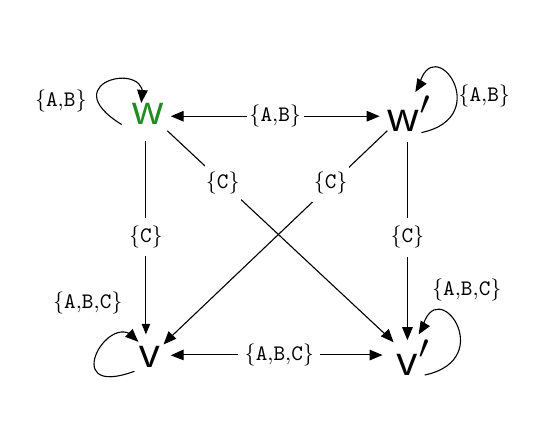
\begin{tikzpicture}[x=0.75pt,y=0.75pt,yscale=-1,xscale=1]
%uncomment if require: \path (0,237.1999969482422); %set diagram left start at 0, and has height of 237.1999969482422

%Straight Lines [id:da49380865843539024] 
\draw    (58,37.52) -- (58,129.88) ;


%Curve Lines [id:da5900505897070274] 
\draw    (55.82,18.4) .. controls (62.62,-2.4) and (11.9,8.32) .. (46.3,29.52) ;


%Shape: Triangle [id:dp7638941010979212] 
\draw  [fill={rgb, 255:red, 0; green, 0; blue, 0 }  ,fill opacity=1 ] (55.82,18.4) -- (54.11,12.94) -- (58.52,13.35) -- cycle ;
%Curve Lines [id:da33896708594278424] 
\draw    (53.81,133.72) .. controls (41.67,115.51) and (14.49,162.32) .. (52.43,148.41) ;


%Shape: Triangle [id:dp06181068467144124] 
\draw  [fill={rgb, 255:red, 0; green, 0; blue, 0 }  ,fill opacity=1 ] (53.81,133.72) -- (48.46,131.68) -- (51.51,128.48) -- cycle ;
%Straight Lines [id:da3518787636435954] 
\draw    (73.3,140.52) -- (171.3,140.52) ;


%Straight Lines [id:da9419961743422685] 
\draw    (167.3,25.52) -- (73.3,25.52) ;


%Straight Lines [id:da5282217469281014] 
\draw    (184,37.72) -- (184,130.08) ;


%Curve Lines [id:da1255493565606156] 
\draw    (191.12,127.8) .. controls (197.84,99.92) and (228.32,142.6) .. (192.32,150.2) ;


%Shape: Triangle [id:dp330887907957337] 
\draw  [fill={rgb, 255:red, 0; green, 0; blue, 0 }  ,fill opacity=1 ] (189.76,130.06) -- (190.59,124.4) -- (194.38,126.68) -- cycle ;
%Curve Lines [id:da19283464821040464] 
\draw    (189.52,11) .. controls (196.24,-16.88) and (226.72,25.8) .. (190.72,33.4) ;


%Shape: Triangle [id:dp48172892570830794] 
\draw  [fill={rgb, 255:red, 0; green, 0; blue, 0 }  ,fill opacity=1 ] (188.16,13.26) -- (188.99,7.6) -- (192.78,9.88) -- cycle ;
%Shape: Triangle [id:dp06884054633092584] 
\draw  [fill={rgb, 255:red, 0; green, 0; blue, 0 }  ,fill opacity=1 ] (184,132.72) -- (181.79,127.43) -- (186.21,127.44) -- cycle ;
%Shape: Triangle [id:dp349860096054311] 
\draw  [fill={rgb, 255:red, 0; green, 0; blue, 0 }  ,fill opacity=1 ] (171.3,140.58) -- (166.02,142.79) -- (166.02,138.37) -- cycle ;
%Shape: Triangle [id:dp5271852980265475] 
\draw  [fill={rgb, 255:red, 0; green, 0; blue, 0 }  ,fill opacity=1 ] (70.66,140.7) -- (75.94,138.31) -- (75.94,142.73) -- cycle ;
%Shape: Triangle [id:dp36308950352931935] 
\draw  [fill={rgb, 255:red, 0; green, 0; blue, 0 }  ,fill opacity=1 ] (58,129.88) -- (56.3,125.81) -- (59.7,125.81) -- cycle ;
%Shape: Triangle [id:dp1292227483684376] 
\draw  [fill={rgb, 255:red, 0; green, 0; blue, 0 }  ,fill opacity=1 ] (70.66,25.52) -- (75.94,23.31) -- (75.94,27.73) -- cycle ;
%Shape: Triangle [id:dp08607057312201727] 
\draw  [fill={rgb, 255:red, 0; green, 0; blue, 0 }  ,fill opacity=1 ] (169.94,25.52) -- (164.66,27.73) -- (164.66,23.31) -- cycle ;
%Straight Lines [id:da22782472852235425] 
\draw    (68.3,32.51) -- (176.84,133.88) ;


%Straight Lines [id:da40972295623496247] 
\draw    (174.3,32.51) -- (68.8,133.01) ;


%Shape: Triangle [id:dp9557525693039122] 
\draw  [fill={rgb, 255:red, 0; green, 0; blue, 0 }  ,fill opacity=1 ] (176.84,133.88) -- (171.64,131.49) -- (174.89,128.49) -- cycle ;
%Shape: Triangle [id:dp9360830131568407] 
\draw  [fill={rgb, 255:red, 0; green, 0; blue, 0 }  ,fill opacity=1 ] (66.99,134.94) -- (69,129.58) -- (72.22,132.61) -- cycle ;

% Text Node
\draw (59,24.32) node [scale=1.7280000000000002] [align=left] {\emphColorSlide{\poss{w}}};
% Text Node
\draw (59.8,141.22) node [scale=1.7280000000000002] [align=left] {\poss{v}};
% Text Node
\draw (17,18.32) node [scale=0.8] [align=left] {\{\agentSlide{A},\agentSlide{B}\}};
% Text Node
\draw (30,115.32) node [scale=0.8] [align=left] {\{\agentSlide{A},\agentSlide{B},\agentSlide{C}\}};
% Text Node
\draw (185.2,24.32) node [scale=1.7280000000000002] [align=left] {\poss{w'}};
% Text Node
\draw (187.11,141.72) node [scale=1.7280000000000002] [align=left] {\poss{v'}};
% Text Node
\draw (212.6,109.32) node [scale=0.8] [align=left] {\{\agentSlide{A},\agentSlide{B},\agentSlide{C}\}};
% Text Node
\draw (221,15.52) node [scale=0.8] [align=left] {\{\agentSlide{A},\agentSlide{B}\}};
% Text Node
\draw  [color={rgb, 255:red, 255; green, 255; blue, 255 }  ,draw opacity=1 ][fill={rgb, 255:red, 255; green, 255; blue, 255 }  ,fill opacity=1 ]  (106.8,16.52) -- (133.8,16.52) -- (133.8,34.52) -- (106.8,34.52) -- cycle  ;
\draw (120.3,25.52) node [scale=0.8,color={rgb, 255:red, 0; green, 0; blue, 0 }  ,opacity=1 ] [align=left] {\{\agentSlide{A},\agentSlide{B}\}};
% Text Node
\draw  [color={rgb, 255:red, 255; green, 255; blue, 255 }  ,draw opacity=1 ][fill={rgb, 255:red, 255; green, 255; blue, 255 }  ,fill opacity=1 ]  (49.5,74.7) -- (66.5,74.7) -- (66.5,92.7) -- (49.5,92.7) -- cycle  ;
\draw (58,83.7) node [scale=0.8,color={rgb, 255:red, 0; green, 0; blue, 0 }  ,opacity=1 ] [align=left] {\{\agentSlide{C}\}};
% Text Node
\draw  [color={rgb, 255:red, 255; green, 255; blue, 255 }  ,draw opacity=1 ][fill={rgb, 255:red, 255; green, 255; blue, 255 }  ,fill opacity=1 ]  (175.5,74.9) -- (192.5,74.9) -- (192.5,92.9) -- (175.5,92.9) -- cycle  ;
\draw (184,83.9) node [scale=0.8,color={rgb, 255:red, 0; green, 0; blue, 0 }  ,opacity=1 ] [align=left] {\{\agentSlide{C}\}};
% Text Node
\draw  [color={rgb, 255:red, 255; green, 255; blue, 255 }  ,draw opacity=1 ][fill={rgb, 255:red, 255; green, 255; blue, 255 }  ,fill opacity=1 ]  (86.5,48.7) -- (103.5,48.7) -- (103.5,66.7) -- (86.5,66.7) -- cycle  ;
\draw (95,57.7) node [scale=0.8,color={rgb, 255:red, 0; green, 0; blue, 0 }  ,opacity=1 ] [align=left] {\{\agentSlide{C}\}};
% Text Node
\draw  [color={rgb, 255:red, 255; green, 255; blue, 255 }  ,draw opacity=1 ][fill={rgb, 255:red, 255; green, 255; blue, 255 }  ,fill opacity=1 ]  (138.5,48.7) -- (155.5,48.7) -- (155.5,66.7) -- (138.5,66.7) -- cycle  ;
\draw (147,57.7) node [scale=0.8,color={rgb, 255:red, 0; green, 0; blue, 0 }  ,opacity=1 ] [align=left] {\{\agentSlide{C}\}};
% Text Node
\draw  [color={rgb, 255:red, 255; green, 255; blue, 255 }  ,draw opacity=1 ][fill={rgb, 255:red, 255; green, 255; blue, 255 }  ,fill opacity=1 ]  (102.8,131.52) -- (141.8,131.52) -- (141.8,149.52) -- (102.8,149.52) -- cycle  ;
\draw (122.3,140.52) node [scale=0.8,color={rgb, 255:red, 0; green, 0; blue, 0 }  ,opacity=1 ] [align=left] {\{\agentSlide{A},\agentSlide{B},\agentSlide{C}\}};


\end{tikzpicture}
}

				}%
			}%
		\end{figure}%
		\begin{center}
			{\footnotesize \transparent{0.8} \Pos\ \emphSlide{\poss{w}} expanded for clarity}
		\end{center}
	}
\end{frame}

\begin{frame}{State equality}
	\begin{itemize}
		\item[-] \PosS\ captures classes of bisimilar Kripke structures
		\item[-] \PosS\ {equality} considers bisimilarity
		\item[-] This help for the \emphSlide{visited states} problem in \mep
	\end{itemize}
	\vfill
	\onslide<2->{
		%\ttSlide{$$\Delta = \peek{B};\distract{B}{C};\flip{C};\tell{B}{C}$$}
		{\footnotesize{\begin{center}
  \poss{r_1}=\bra{
    (\agentSlide{A}, \bra{\poss{s_0}, \poss{s_1}}),
    (\agentSlide{B}, \bra{\poss r_1}),
    (\agentSlide{C}, \bra{\poss r_1}),
    \ttSlide{look(\agentSlide{C})},
    \ttSlide{key(\agentSlide{A})},
	\ttSlide{opened},
	\ttSlide{heads}
}
\end{center}
}}
		\begin{figure}
			\centering
			{\scalebox{.37}{\input{img/equality1_corr}}}
			\hfill
			{\scalebox{0.37}{\tikzset{every picture/.style={line width=0.75pt}} %set default line width to 0.75pt        
\trimbox{0cm 0cm 0cm 1.8cm}{ 
\begin{tikzpicture}[x=0.75pt,y=0.75pt,yscale=-1,xscale=1]
%uncomment if require: \path (0,332); %set diagram left start at 0, and has height of 332

%Shape: Circle [id:dp09506861109760789] 
\draw   (67.5,279.5) .. controls (67.5,262.66) and (81.16,249) .. (98,249) .. controls (114.84,249) and (128.5,262.66) .. (128.5,279.5) .. controls (128.5,296.34) and (114.84,310) .. (98,310) .. controls (81.16,310) and (67.5,296.34) .. (67.5,279.5) -- cycle ;
%Shape: Circle [id:dp3674876277032001] 
\draw   (240.5,279.5) .. controls (240.5,262.66) and (254.16,249) .. (271,249) .. controls (287.84,249) and (301.5,262.66) .. (301.5,279.5) .. controls (301.5,296.34) and (287.84,310) .. (271,310) .. controls (254.16,310) and (240.5,296.34) .. (240.5,279.5) -- cycle ;
%Straight Lines [id:da686791560478396] 
\draw    (131,279.5) -- (238.5,279.5) ;
\draw [shift={(240.5,279.5)}, rotate = 180] [fill={rgb, 255:red, 0; green, 0; blue, 0 }  ][line width=0.75]  [draw opacity=0] (8.93,-4.29) -- (0,0) -- (8.93,4.29) -- cycle    ;
\draw [shift={(129,279.5)}, rotate = 0] [fill={rgb, 255:red, 0; green, 0; blue, 0 }  ][line width=0.75]  [draw opacity=0] (8.93,-4.29) -- (0,0) -- (8.93,4.29) -- cycle    ;
%Curve Lines [id:da3133467592132765] 
\draw    (67.5,279.5) .. controls (-31.5,263.58) and (50.67,180.83) .. (89.42,247.48) ;
\draw [shift={(90,248.5)}, rotate = 240.66] [fill={rgb, 255:red, 0; green, 0; blue, 0 }  ][line width=0.75]  [draw opacity=0] (8.93,-4.29) -- (0,0) -- (8.93,4.29) -- cycle    ;

%Curve Lines [id:da09866336174690571] 
\draw    (301.5,279.5) .. controls (391.91,267.58) and (313.16,179.07) .. (280.98,249.43) ;
\draw [shift={(280.5,250.5)}, rotate = 293.78] [fill={rgb, 255:red, 0; green, 0; blue, 0 }  ][line width=0.75]  [draw opacity=0] (8.93,-4.29) -- (0,0) -- (8.93,4.29) -- cycle    ;

%Shape: Circle [id:dp9019764791073822] 
\draw  [fill={rgb, 255:red, 0; green, 0; blue, 0 }  ,fill opacity=1 ] (240.5,73.5) .. controls (240.5,56.66) and (254.16,43) .. (271,43) .. controls (287.84,43) and (301.5,56.66) .. (301.5,73.5) .. controls (301.5,90.34) and (287.84,104) .. (271,104) .. controls (254.16,104) and (240.5,90.34) .. (240.5,73.5) -- cycle ;
%Shape: Circle [id:dp23164546006052256] 
\draw  [fill={rgb, 255:red, 255; green, 255; blue, 255 }  ,fill opacity=1 ] (246,73.5) .. controls (246,59.69) and (257.19,48.5) .. (271,48.5) .. controls (284.81,48.5) and (296,59.69) .. (296,73.5) .. controls (296,87.31) and (284.81,98.5) .. (271,98.5) .. controls (257.19,98.5) and (246,87.31) .. (246,73.5) -- cycle ;
%Straight Lines [id:da3406951202857561] 
\draw    (255.5,96.5) -- (112.48,251.28) ;
\draw [shift={(111.13,252.75)}, rotate = 312.74] [fill={rgb, 255:red, 0; green, 0; blue, 0 }  ][line width=0.75]  [draw opacity=0] (8.93,-4.29) -- (0,0) -- (8.93,4.29) -- cycle    ;

%Straight Lines [id:da5969218919849798] 
\draw    (271,104) -- (271,247) ;
\draw [shift={(271,249)}, rotate = 270] [fill={rgb, 255:red, 0; green, 0; blue, 0 }  ][line width=0.75]  [draw opacity=0] (8.93,-4.29) -- (0,0) -- (8.93,4.29) -- cycle    ;

%Curve Lines [id:da32162073734028385] 
\draw    (296.5,72.5) .. controls (386.91,60.58) and (308.16,-27.93) .. (275.98,42.43) ;
\draw [shift={(275.5,43.5)}, rotate = 293.78] [fill={rgb, 255:red, 0; green, 0; blue, 0 }  ][line width=0.75]  [draw opacity=0] (8.93,-4.29) -- (0,0) -- (8.93,4.29) -- cycle    ;


% Text Node
\draw  [color={rgb, 255:red, 255; green, 255; blue, 255 }  ,draw opacity=1 ][fill={rgb, 255:red, 255; green, 255; blue, 255 }  ,fill opacity=1 ]  (155.75,267.5) -- (213.75,267.5) -- (213.75,291.5) -- (155.75,291.5) -- cycle  ;
\draw (184.75,279.5) node   {\{\agentSlide{A},\agentSlide{B},\agentSlide{C}\}};
% Text Node
\draw (98,279.5) node   {\defemph{s_{0}}};
% Text Node
\draw (271,279.5) node   {\defemph{s_{1}}};
% Text Node
\draw  [color={rgb, 255:red, 255; green, 255; blue, 255 }  ,draw opacity=1 ][fill={rgb, 255:red, 255; green, 255; blue, 255 }  ,fill opacity=1 ]  (16,219.5) -- (74,219.5) -- (74,243.5) -- (16,243.5) -- cycle  ;
\draw (45,231.5) node   {\{\agentSlide{A},\agentSlide{B},\agentSlide{C}\}};
% Text Node
\draw  [color={rgb, 255:red, 255; green, 255; blue, 255 }  ,draw opacity=1 ][fill={rgb, 255:red, 255; green, 255; blue, 255 }  ,fill opacity=1 ]  (290,214.5) -- (348,214.5) -- (348,238.5) -- (290,238.5) -- cycle  ;
\draw (319,226.5) node   {\{\agentSlide{A},\agentSlide{B},\agentSlide{C}\}};
% Text Node
\draw (271,73.5) node   {\defemph{r_{1}}};
% Text Node
\draw  [color={rgb, 255:red, 255; green, 255; blue, 255 }  ,draw opacity=1 ][fill={rgb, 255:red, 255; green, 255; blue, 255 }  ,fill opacity=1 ]  (217.5,112.5) -- (238.5,112.5) -- (238.5,136.5) -- (217.5,136.5) -- cycle  ;
\draw (228,124.5) node   {\{\agentSlide{A}\}};
% Text Node
\draw  [color={rgb, 255:red, 255; green, 255; blue, 255 }  ,draw opacity=1 ][fill={rgb, 255:red, 255; green, 255; blue, 255 }  ,fill opacity=1 ]  (261,130.5) -- (282,130.5) -- (282,154.5) -- (261,154.5) -- cycle  ;
\draw (271.5,142.5) node   {\{\agentSlide{A}\}};
% Text Node
\draw  [color={rgb, 255:red, 255; green, 255; blue, 255 }  ,draw opacity=1 ][fill={rgb, 255:red, 255; green, 255; blue, 255 }  ,fill opacity=1 ]  (321,22.5) -- (359,22.5) -- (359,46.5) -- (321,46.5) -- cycle  ;
\draw (340,34.5) node   {\{\agentSlide{B},\agentSlide{C}\}};


\end{tikzpicture}}}}
		\end{figure}
	}
\end{frame}

\subsection*{Entailment}
\begin{frame}{Entailment}
	Let $\varphi,\varphi_{1},\varphi_{2}$ be beliefs formula and \poss{u} be a \pos
	\begin{block}{Entailment w.r.t. \posS}
			\begin{itemize}[<+->]
			\item[-] $\poss{u} \models \ttSlide{l}$ if $\possarg{u}{\ttSlide{l}}= 1$;
			%\item $\poss{u} \models \neg \phi$ if $\poss{u} \not \models \phi$;
			%\item $\poss{u} \models \phi_1 \vee \phi_2$ if $\poss{u} \models
			%	      \phi_1$ or $\poss{u} \models \phi_2$;
			%\item $\poss{u} \models \phi_1 \wedge \phi_2$ if $\poss{u} \models
			%	      \phi_1$ and $\poss{u} \models \phi_2$.
			\item[-] $\poss{u} \models \bBSlide{\agentSlide{ag}}{\varphi}$ if for each $\poss{v} \in \possarg{u}{\agentSlide{ag}}$, $\poss{v} \models \varphi$;
			      %\item $\poss{u} \models \neg \varphi$ if $\poss{u} \not\models \varphi$;
		%	\item $\poss{u} \models \varphi_1 \vee \varphi_2$ if $\poss{u} \models \varphi_1$ or $\poss{u}\models \varphi_2$;
		%	\item $\poss{u} \models \varphi_1 \wedge \varphi_2$ if $\poss{u} \models \varphi_1$ and $\poss{u}\models \varphi_2$;
			\item[-] $\poss{u} \models \eAlpha{\varphi}$ if $\poss{u} \models
				      \bB{ag}{\varphi}$ for all $\agentSlide{ag} \in \alpha$;
			\item<.->[-] $\poss{u} \models \cAlpha{\varphi}$ if
			      $\poss{u} \models \eAlphaIter{k}{\varphi}$ for every
			      $k\geq0$, where $\eAlphaIter{0}{\varphi} = \varphi$ and
			      $\eAlphaIter{k+1}{\varphi}=\eAlpha{(\eAlphaIter{k}{\varphi})}$.
		\end{itemize}
	\end{block}
		\onslide<3->{The entailment for the standard operators is defined as usual}
\end{frame}

\subsection*{Transition function}
\begin{frame}{Ontic Actions}
	
	\begin{block}{$\trfunc$ for Ontic Actions \hfill $\trfunc: \ai\times\Sigma \rightarrow \Sigma \cup \bra{\emptyset}$}
	
	Let \texttt{a} be an \emphSlide{ontic action} instance, \poss{u} a \pos\ and \ttSlide{l} be \ttSlide{f} or \ttSlide{$\neg$}\ttSlide{f}\\
			\vspace{0.2cm}
	\begin{tabular}{rl}
		$\trfunc(\texttt{a}, \poss{u}) =  \emptyset$ &if \texttt{a} is not executable in \poss{u}\\
		$\trfunc( \texttt{a}, \poss{u}) = \poss{v}$& if \texttt{a} \emphSlide{modifies} the \ttSlide{literals} $\in$ \res{a}\\
	\end{tabular}
	
	\vspace{0.65cm}
	Where \poss{v} is\\
		\vspace{0.2cm}
		      $\begin{cases}
				      \possarg{v}{\ttSlide{l}} = \possarg{u}{\ttSlide{l}} & \text{ if } \ttSlide{l} \not\in \res{a} \\
				      \possarg{v}{\ttSlide{l}} = \resSlide{a}{l}                  & \text{ if } \ttSlide{l} \in \res{a}  
				      %\res a &\text{ if } \defemph{f} \in \res{a}
			      \end{cases}$
		      \vspace*{0.2cm}
		      \\and
		      \vspace*{0.2cm}
		      \\
		      $\begin{cases}
				      \possarg{v}{\agentSlide{ag}} = \possarg{u}{\agentSlide{ag}}                                                        & \text{ if } \agentSlide{ag} \in \posoblivious \\
				      \possarg{v}{\agentSlide{ag}} = \bigcup_{\poss{w} \in \possarg{u}{\agentSlide{ag}}} \trfunc( \texttt{a}, \poss{w}) & \text{ if } \agentSlide{ag} \in \posfull
			      \end{cases}$
			    \end{block}

\end{frame}


\begin{frame}{Sensing Actions}
	
	\begin{block}{$\trfunc$ for Sensing Actions \hfill $\trfunc: \ai\times\Sigma \rightarrow \Sigma \cup \bra{\emptyset}$}
		
		Let \texttt{a} be an \emphSlide{sensing action} instance, and \poss{u} a \pos\  and \ttSlide{l} be \ttSlide{f} or \ttSlide{$\neg$}\ttSlide{f}\\
		\vspace{0.2cm}
		\begin{tabular}{rl}
			$\trfunc(\texttt{a}, \poss{u}) =  \emptyset$ &if \texttt{a} is not executable in \poss{u}\\
			$\trfunc( \texttt{a}, \poss{u}) = \poss{v}$& if the literal \ttSlide{l} is \emphSlide{sensed}\\
		\end{tabular}
		
		\vspace{0.65cm}
		Where \poss{v} is\\
		\vspace{0.2cm}
		$\begin{cases}
		\emptyset & \text{if } \sensedSlide{a}{l} \neq \possarg{u}{\ttSlide{l}}\\
		\possarg{v}{\agentSlide{ag}} = \possarg{u}{\agentSlide{ag}}                                                                                                   & \text{if } \agentSlide{ag} \in \posoblivious\\
		\possarg{v}{\agentSlide{ag}} = \bigcup_{\poss{w} \in \possarg{u}{\agentSlide{ag}}} \trfunc( \defemph{a}, \poss{w}) & \text{if }\agentSlide{ag} \in \posfull\\
		\possarg{v}{\agentSlide{ag}} = \bigcup_{\poss{w} \in \possarg{u}{\agentSlide{ag}}} (\trfunc( \defemph{a}, \poss{w}) \cup \trfunc( \neg\defemph{a}, \poss{w})) & \text{if }\agentSlide{ag} \in \pospartial
		\end{cases}$
	\end{block}
	
\end{frame}


\begin{frame}{Announcement Actions}
	
	\begin{block}{$\trfunc$ for Announcement Actions \hfill $\trfunc: \ai\times\Sigma \rightarrow \Sigma \cup \bra{\emptyset}$}
		
		Let \texttt{a} be an \emphSlide{announcement action} instance, and \poss{u} a \pos.\\
		\vspace{0.2cm}
		\begin{tabular}{rl}
			$\trfunc(\texttt{a}, \poss{u}) =  \emptyset$ &if \texttt{a} is not executable in \poss{u}\\
			$\trfunc( \texttt{a}, \poss{u}) = \poss{v}$& if the fluent formula \ttSlide{$\phi$} is \emphSlide{announced}\\
		\end{tabular}
		
		\vspace{0.65cm}
		Where \poss{v} is\\
		\vspace{0.2cm}
		$\begin{cases}
	\emptyset & \text{if } \poss{u} \not \models \phi\\
		\possarg{v}{\agentSlide{ag}} = \possarg{u}{\agentSlide{ag}}                                                                                                   & \text{if } \agentSlide{ag} \in \posoblivious\\
		\possarg{v}{\agentSlide{ag}} = \bigcup_{\poss{w} \in \possarg{u}{\agentSlide{ag}}} \trfunc( \defemph{a}, \poss{w}) & \text{if }\agentSlide{ag} \in \posfull\\
		\possarg{v}{\agentSlide{ag}} = \bigcup_{\poss{w} \in \possarg{u}{\agentSlide{ag}}} (\trfunc( \defemph{a}, \poss{w}) \cup \trfunc( \neg\defemph{a}, \poss{w})) & \text{if }\agentSlide{ag} \in \pospartial
		\end{cases}$
	\end{block}
	
\end{frame}
%\section{Example}
\section{Conclusions}

\subsection*{Future works}
\begin{frame}{Conclusions}
	\begin{itemize}
		\item[-] Exploited an \emphSlide{alternative} to  the \emph{Kripke structures} as states representation
		\item[-] Used \emph{\posS}\ to define a stronger concept of states \emphSlide{equality}
		\item[-] \PosS\ helps in  \emphSlide{reducing} the search-space dimension
		\item[-] Defined a new action language for the \mep\ problem
	\end{itemize}
\end{frame}

\begin{frame}{Future works}

	\begin{itemize}
		\item[-] We started \emphSlide{implementing} a planner for \ourL\vspace{0.5cm}
		\itemsep0.3cm
		\item[-] Exploit more \emphSlide{set-based operations}: especially for the entailment of group operators
		\item[-] Formalize the concept of \emphSlide{non-consistent belief} for \ourL
		      %\item Investigate more thoroughly the \emphSlide{connection} between Kripke structures and \nwf\ sets
		      %\item Examine the concept of \emphSlide{bisimulation} as \emphSlide{equality} between epistemic states
		\item[-] Consider other \emphSlide{alternatives} to Kripke structures, \eg \emphSlide{OBDD}s
	\end{itemize}
\end{frame}


\begin{frame}{The end}
	\begin{columns}
		\begin{column}{0.5\textwidth}
			\begin{center}
				\includegraphics[width=0.5\textwidth]{img/QandA_charlie2}
			\end{center}
		\end{column}
		\begin{column}{0.5\textwidth}
			\begin{center}
				\centering {\Large \emphSlide{\textbf{Thank You\\ for the attention}}}
			\end{center}
		\end{column}
	\end{columns}
\end{frame}

%No page Numbering
\setbeamercolor{headline}{fg=white,bg=black}
\setbeamertemplate{headline}{
	\begin{beamercolorbox}[wd=1.0\paperwidth,left,ht=38pt,dp=1ex]{headline}
	\end{beamercolorbox}
	\vspace*{2.3pt}
	\color{black!30!white}\rule{\paperwidth}{2pt}
}

%BIBLIOGRAPHY


\showCILC{true}{\begin{frame}[allowframebreaks,noframenumbering]{References}
	\printbibliography
\end{frame}}

\appendix

\section*{Backup Slides}
\begin{frame}[noframenumbering]{Side to side Execution}
	\begin{center}
		\begin{figure}%[H]
				\begin{subfigure}{0.5\textwidth}
					\hspace*{-0.6cm}\scalebox{.5}%
					{%
						\raisebox{0.5cm}{
							\only<1>{

\tikzset{every picture/.style={line width=0.75pt}} %set default line width to 0.75pt        
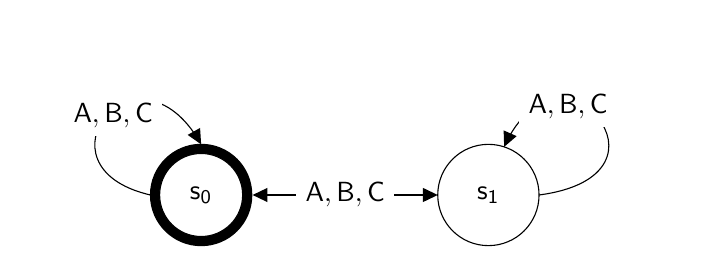
\begin{tikzpicture}[x=0.75pt,y=0.75pt,yscale=-0.8,xscale=0.8]
%uncomment if require: \path (0,150); %set diagram left start at 0, and has height of 150

%Shape: Circle [id:dp4325934269433842] 
\draw  [fill={rgb, 255:red, 0; green, 0; blue, 0 }  ,fill opacity=1 ] (216.5,93) .. controls (216.5,76.16) and (230.16,62.5) .. (247,62.5) .. controls (263.84,62.5) and (277.5,76.16) .. (277.5,93) .. controls (277.5,109.84) and (263.84,123.5) .. (247,123.5) .. controls (230.16,123.5) and (216.5,109.84) .. (216.5,93) -- cycle ;
%Shape: Circle [id:dp8959340303758652] 
\draw   (389.5,93) .. controls (389.5,76.16) and (403.16,62.5) .. (420,62.5) .. controls (436.84,62.5) and (450.5,76.16) .. (450.5,93) .. controls (450.5,109.84) and (436.84,123.5) .. (420,123.5) .. controls (403.16,123.5) and (389.5,109.84) .. (389.5,93) -- cycle ;
%Straight Lines [id:da6159546739572547] 
\draw    (280,93) -- (387.5,93) ;
\draw [shift={(389.5,93)}, rotate = 180] [fill={rgb, 255:red, 0; green, 0; blue, 0 }  ][line width=0.75]  [draw opacity=0] (8.93,-4.29) -- (0,0) -- (8.93,4.29) -- cycle    ;
\draw [shift={(278,93)}, rotate = 0] [fill={rgb, 255:red, 0; green, 0; blue, 0 }  ][line width=0.75]  [draw opacity=0] (8.93,-4.29) -- (0,0) -- (8.93,4.29) -- cycle    ;
%Curve Lines [id:da8452234444075793] 
\draw    (216.5,93) .. controls (142.87,76.08) and (207.84,-5.18) .. (246.42,61.48) ;
\draw [shift={(247,62.5)}, rotate = 240.66] [fill={rgb, 255:red, 0; green, 0; blue, 0 }  ][line width=0.75]  [draw opacity=0] (8.93,-4.29) -- (0,0) -- (8.93,4.29) -- cycle    ;

%Curve Lines [id:da8370233876099651] 
\draw    (450.5,93) .. controls (540.91,81.08) and (462.16,-7.43) .. (429.98,62.93) ;
\draw [shift={(429.5,64)}, rotate = 293.78] [fill={rgb, 255:red, 0; green, 0; blue, 0 }  ][line width=0.75]  [draw opacity=0] (8.93,-4.29) -- (0,0) -- (8.93,4.29) -- cycle    ;

%Shape: Circle [id:dp08152116050102409] 
\draw  [fill={rgb, 255:red, 255; green, 255; blue, 255 }  ,fill opacity=1 ] (222,93) .. controls (222,79.19) and (233.19,68) .. (247,68) .. controls (260.81,68) and (272,79.19) .. (272,93) .. controls (272,106.81) and (260.81,118) .. (247,118) .. controls (233.19,118) and (222,106.81) .. (222,93) -- cycle ;

% Text Node
\draw  [color={rgb, 255:red, 255; green, 255; blue, 255 }  ,draw opacity=1 ][fill={rgb, 255:red, 255; green, 255; blue, 255 }  ,fill opacity=1 ]  (304.75,81) -- (362.75,81) -- (362.75,105) -- (304.75,105) -- cycle  ;
\draw (333.75,93) node   {$\agent{A}, \agent{B}, \agent{C}$};
% Text Node
\draw (247,93) node   {$\defemph{s_0}$};
% Text Node
\draw (420,93) node   {$\defemph{s_1}$};
% Text Node
\draw  [color={rgb, 255:red, 255; green, 255; blue, 255 }  ,draw opacity=1 ][fill={rgb, 255:red, 255; green, 255; blue, 255 }  ,fill opacity=1 ]  (165,33) -- (223,33) -- (223,57) -- (165,57) -- cycle  ;
\draw (194,45) node   {$\agent{A}, \agent{B}, \agent{C}$};
% Text Node
\draw  [color={rgb, 255:red, 255; green, 255; blue, 255 }  ,draw opacity=1 ][fill={rgb, 255:red, 255; green, 255; blue, 255 }  ,fill opacity=1 ]  (439,28) -- (497,28) -- (497,52) -- (439,52) -- cycle  ;
\draw (468,40) node   {$\agent{A}, \agent{B}, \agent{C}$};

%\draw (340,160) node   {%
%	$\begin{aligned}
%	\interp{0}{s_0}&=\bra{\looking {AG}, \haskey A}\\
%	\interp{0}{s_1}&=\bra{\looking {AG}, \haskey{A}, \head}
%	\end{aligned}$
%	\hspace*{0.2cm}where \agent{ag} $\in$ \bra{\agent{a}, \agent{b}, \agent{c}}.};

\end{tikzpicture}

}
							\only<2>{\input{img/appendix/distract_state_kripke}}
							\only<3>{

\tikzset{every picture/.style={line width=0.75pt}} %set default line width to 0.75pt        

\begin{tikzpicture}[x=0.75pt,y=0.75pt,yscale=-1,xscale=1]
%uncomment if require: \path (0,371); %set diagram left start at 0, and has height of 371

%Shape: Circle [id:dp4325934269433842] 
\draw   (171.5,287) .. controls (171.5,270.16) and (185.16,256.5) .. (202,256.5) .. controls (218.84,256.5) and (232.5,270.16) .. (232.5,287) .. controls (232.5,303.84) and (218.84,317.5) .. (202,317.5) .. controls (185.16,317.5) and (171.5,303.84) .. (171.5,287) -- cycle ;
%Shape: Circle [id:dp8959340303758652] 
\draw   (344.5,287) .. controls (344.5,270.16) and (358.16,256.5) .. (375,256.5) .. controls (391.84,256.5) and (405.5,270.16) .. (405.5,287) .. controls (405.5,303.84) and (391.84,317.5) .. (375,317.5) .. controls (358.16,317.5) and (344.5,303.84) .. (344.5,287) -- cycle ;
%Straight Lines [id:da6159546739572547] 
\draw    (235,287) -- (342.5,287) ;
\draw [shift={(344.5,287)}, rotate = 180] [fill={rgb, 255:red, 0; green, 0; blue, 0 }  ][line width=0.75]  [draw opacity=0] (8.93,-4.29) -- (0,0) -- (8.93,4.29) -- cycle    ;
\draw [shift={(233,287)}, rotate = 0] [fill={rgb, 255:red, 0; green, 0; blue, 0 }  ][line width=0.75]  [draw opacity=0] (8.93,-4.29) -- (0,0) -- (8.93,4.29) -- cycle    ;
%Curve Lines [id:da8452234444075793] 
\draw    (171.5,287) .. controls (72.5,271.08) and (154.67,188.33) .. (193.42,254.98) ;
\draw [shift={(194,256)}, rotate = 240.66] [fill={rgb, 255:red, 0; green, 0; blue, 0 }  ][line width=0.75]  [draw opacity=0] (8.93,-4.29) -- (0,0) -- (8.93,4.29) -- cycle    ;

%Curve Lines [id:da8370233876099651] 
\draw    (405.5,287) .. controls (495.91,275.08) and (417.16,186.57) .. (384.98,256.93) ;
\draw [shift={(384.5,258)}, rotate = 293.78] [fill={rgb, 255:red, 0; green, 0; blue, 0 }  ][line width=0.75]  [draw opacity=0] (8.93,-4.29) -- (0,0) -- (8.93,4.29) -- cycle    ;

%Shape: Circle [id:dp7932635156571649] 
\draw  [fill={rgb, 255:red, 0; green, 0; blue, 0 }  ,fill opacity=1 ] (172.5,104) .. controls (172.5,87.16) and (186.16,73.5) .. (203,73.5) .. controls (219.84,73.5) and (233.5,87.16) .. (233.5,104) .. controls (233.5,120.84) and (219.84,134.5) .. (203,134.5) .. controls (186.16,134.5) and (172.5,120.84) .. (172.5,104) -- cycle ;
%Shape: Circle [id:dp6105058367437692] 
\draw   (345.5,104) .. controls (345.5,87.16) and (359.16,73.5) .. (376,73.5) .. controls (392.84,73.5) and (406.5,87.16) .. (406.5,104) .. controls (406.5,120.84) and (392.84,134.5) .. (376,134.5) .. controls (359.16,134.5) and (345.5,120.84) .. (345.5,104) -- cycle ;
%Straight Lines [id:da9340669325180512] 
\draw    (236,104) -- (343.5,104) ;
\draw [shift={(345.5,104)}, rotate = 180] [fill={rgb, 255:red, 0; green, 0; blue, 0 }  ][line width=0.75]  [draw opacity=0] (8.93,-4.29) -- (0,0) -- (8.93,4.29) -- cycle    ;
\draw [shift={(234,104)}, rotate = 0] [fill={rgb, 255:red, 0; green, 0; blue, 0 }  ][line width=0.75]  [draw opacity=0] (8.93,-4.29) -- (0,0) -- (8.93,4.29) -- cycle    ;
%Curve Lines [id:da4572197115547698] 
\draw    (172.5,104) .. controls (98.87,87.08) and (163.84,5.82) .. (202.42,72.48) ;
\draw [shift={(203,73.5)}, rotate = 240.66] [fill={rgb, 255:red, 0; green, 0; blue, 0 }  ][line width=0.75]  [draw opacity=0] (8.93,-4.29) -- (0,0) -- (8.93,4.29) -- cycle    ;

%Curve Lines [id:da9119172492888147] 
\draw    (406.5,104) .. controls (496.91,92.08) and (418.16,3.57) .. (385.98,73.93) ;
\draw [shift={(385.5,75)}, rotate = 293.78] [fill={rgb, 255:red, 0; green, 0; blue, 0 }  ][line width=0.75]  [draw opacity=0] (8.93,-4.29) -- (0,0) -- (8.93,4.29) -- cycle    ;

%Shape: Circle [id:dp47196260233615805] 
\draw  [fill={rgb, 255:red, 255; green, 255; blue, 255 }  ,fill opacity=1 ] (178,104) .. controls (178,90.19) and (189.19,79) .. (203,79) .. controls (216.81,79) and (228,90.19) .. (228,104) .. controls (228,117.81) and (216.81,129) .. (203,129) .. controls (189.19,129) and (178,117.81) .. (178,104) -- cycle ;
%Straight Lines [id:da04653031760639226] 
\draw    (222.75,125.5) -- (357.09,260.58) ;
\draw [shift={(358.5,262)}, rotate = 225.16] [fill={rgb, 255:red, 0; green, 0; blue, 0 }  ][line width=0.75]  [draw opacity=0] (8.93,-4.29) -- (0,0) -- (8.93,4.29) -- cycle    ;

%Straight Lines [id:da7004759142531133] 
\draw    (362.13,131.25) -- (216.63,258.93) ;
\draw [shift={(215.13,260.25)}, rotate = 318.73] [fill={rgb, 255:red, 0; green, 0; blue, 0 }  ][line width=0.75]  [draw opacity=0] (8.93,-4.29) -- (0,0) -- (8.93,4.29) -- cycle    ;

%Straight Lines [id:da7971203391650094] 
\draw    (203,134.5) -- (202.02,254.5) ;
\draw [shift={(202,256.5)}, rotate = 270.47] [fill={rgb, 255:red, 0; green, 0; blue, 0 }  ][line width=0.75]  [draw opacity=0] (8.93,-4.29) -- (0,0) -- (8.93,4.29) -- cycle    ;

%Straight Lines [id:da21593783196193417] 
\draw    (376,134.5) -- (375.02,254.5) ;
\draw [shift={(375,256.5)}, rotate = 270.47] [fill={rgb, 255:red, 0; green, 0; blue, 0 }  ][line width=0.75]  [draw opacity=0] (8.93,-4.29) -- (0,0) -- (8.93,4.29) -- cycle    ;


% Text Node
\draw  [color={rgb, 255:red, 255; green, 255; blue, 255 }  ,draw opacity=1 ][fill={rgb, 255:red, 255; green, 255; blue, 255 }  ,fill opacity=1 ]  (259.75,275) -- (317.75,275) -- (317.75,299) -- (259.75,299) -- cycle  ;
\draw (288.75,287) node   {\{$\agentSlide{A},\agentSlide{B},\agentSlide{C}$\}};
% Text Node
\draw (202,287) node   {\defemph{p_{0}}};
% Text Node
\draw (375,287) node   {\defemph{p_{1}}};
% Text Node
\draw  [color={rgb, 255:red, 255; green, 255; blue, 255 }  ,draw opacity=1 ][fill={rgb, 255:red, 255; green, 255; blue, 255 }  ,fill opacity=1 ]  (120,227) -- (178,227) -- (178,251) -- (120,251) -- cycle  ;
\draw (149,239) node   {\{$\agentSlide{A}, \agentSlide{B},\agentSlide{C}$\}};
% Text Node
\draw  [color={rgb, 255:red, 255; green, 255; blue, 255 }  ,draw opacity=1 ][fill={rgb, 255:red, 255; green, 255; blue, 255 }  ,fill opacity=1 ]  (394,222) -- (452,222) -- (452,246) -- (394,246) -- cycle  ;
\draw (423,234) node   {\{$\agentSlide{A},\agentSlide{B},\agentSlide{C}$\}};
% Text Node
\draw  [color={rgb, 255:red, 255; green, 255; blue, 255 }  ,draw opacity=1 ][fill={rgb, 255:red, 255; green, 255; blue, 255 }  ,fill opacity=1 ]  (270.25,92) -- (309.25,92) -- (309.25,116) -- (270.25,116) -- cycle  ;
\draw (289.75,104) node   {\{$\agentSlide{A},\agentSlide{B}$\}};
% Text Node
\draw (203,104) node   {\defemph{q_{0}}};
% Text Node
\draw (376,104) node   {\defemph{q_{1}}};
% Text Node
\draw  [color={rgb, 255:red, 255; green, 255; blue, 255 }  ,draw opacity=1 ][fill={rgb, 255:red, 255; green, 255; blue, 255 }  ,fill opacity=1 ]  (130.5,44) -- (169.5,44) -- (169.5,68) -- (130.5,68) -- cycle  ;
\draw (150,56) node   {\{$\agentSlide{A},\agentSlide{B}$\}};
% Text Node
\draw  [color={rgb, 255:red, 255; green, 255; blue, 255 }  ,draw opacity=1 ][fill={rgb, 255:red, 255; green, 255; blue, 255 }  ,fill opacity=1 ]  (405.5,39) -- (444.5,39) -- (444.5,63) -- (405.5,63) -- cycle  ;
\draw (425,51) node   {\{$\agentSlide{A},\agentSlide{B}$\}};
% Text Node
\draw  [color={rgb, 255:red, 255; green, 255; blue, 255 }  ,draw opacity=1 ][fill={rgb, 255:red, 255; green, 255; blue, 255 }  ,fill opacity=1 ]  (188,174) -- (208,174) -- (208,198) -- (188,198) -- cycle  ;
\draw (198,186) node   {\{$\agentSlide{C}$\}};
% Text Node
\draw  [color={rgb, 255:red, 255; green, 255; blue, 255 }  ,draw opacity=1 ][fill={rgb, 255:red, 255; green, 255; blue, 255 }  ,fill opacity=1 ]  (234,140) -- (254,140) -- (254,164) -- (234,164) -- cycle  ;
\draw (244,152) node   {\{$\agentSlide{C}$\}};
% Text Node
\draw  [color={rgb, 255:red, 255; green, 255; blue, 255 }  ,draw opacity=1 ][fill={rgb, 255:red, 255; green, 255; blue, 255 }  ,fill opacity=1 ]  (327,140) -- (347,140) -- (347,164) -- (327,164) -- cycle  ;
\draw (337,152) node   {\{$\agentSlide{C}$\}};
% Text Node
\draw  [color={rgb, 255:red, 255; green, 255; blue, 255 }  ,draw opacity=1 ][fill={rgb, 255:red, 255; green, 255; blue, 255 }  ,fill opacity=1 ]  (366,175) -- (386,175) -- (386,199) -- (366,199) -- cycle  ;
\draw (376,187) node   {\{$\agentSlide{C}$\}};

\draw (310,380) node   {
							$\begin{aligned}
							\interp{2}{q_0}&=\bra{\ttSlide{look(\agentSlide{ag})}, \ttSlide{key(\agentSlide{A})}, \ttSlide{opened}, \ttSlide{heads}}\\
							\interp{2}{q_1}&=\bra{\ttSlide{look(\agentSlide{ag})}, \ttSlide{key(\agentSlide{A})}, \ttSlide{opened}}\\
							\interp{2}{p_0}&=\interp{1}{p_0}\\
							\interp{2}{p_1}&=\interp{1}{p_1}
						\end{aligned}$};

\end{tikzpicture}

}
							\only<4>{\input{img/appendix/peek_state_kripke}}
						}%
					}%
				\end{subfigure}%
				\begin{subfigure}{0.5\textwidth}
					\hspace*{0.6cm}\scalebox{0.6}%
					{%
						%	\raisebox{1.5cm}{
						\only<1>{
$\begin{cases}
 \poss u &= \bra{(\agentSlide{ag},\bra{\poss{u}, \poss{u^\prime}}),\\
 	&\text{~~~~~}\ttSlide{look(\agentSlide{ag})}, \ttSlide{key(\agentSlide{A})}, \ttSlide{heads}}\\
 \poss u^\prime &= \bra{(\agentSlide{ag},\bra{\poss{u}, \poss{u^\prime}}),\\
 	&\text{~~~~~}\ttSlide{look(\agentSlide{ag})}, \ttSlide{key(\agentSlide{A})}}
\end{cases}$
}
						\only<2>{$
\begin{aligned}
	&\begin{cases}
		\poss{v}&= \bra{
	     	(\agent{ag},\bra{\poss{v}, \poss{v^\prime}}),	\looking{a},
	     	\looking{b},
	     	\haskey{a}%
		}\\
			\poss{v}^\prime&= \bra{
	    	(\agent{ag},\bra{\poss{v}, \poss{v^\prime}}),
	    	\looking{a},
	    	\looking{b},
	    	\haskey{a},
	    	\head%
		}\\
	\end{cases}\\
	&\text{where }  \agent{ag}  \in \bra{\agent{A}, \agent{B}, \agent{C}}
\end{aligned}
$


}
						\only<3>{$\begin{aligned}
  &\begin{cases}
    \poss{w}&= \bra{
      (\agentSlide{ag},\bra{\poss{w}, \poss{w^\prime}}),
      (\agentSlide{c},\bra{\poss{v}, \poss{v^\prime}}),\\
      &\text{~~~~~}\ttSlide{look(\agentSlide{ag})},
      \ttSlide{key(\agentSlide{A})},
      \ttSlide{opened}, \ttSlide{heads}}\\
    \poss{w^\prime} &=\bra{
      (\agentSlide{ag},\bra{\poss{w}, \poss{w^\prime}}),
      (\agentSlide{c},\bra{\poss{v}, \poss{v^\prime}}),\\
      &\text{~~~~~}\ttSlide{look(\agentSlide{ag})}, \ttSlide{key(\agentSlide{A})}, \ttSlide{opened}}
   \end{cases}\\
  &\text{where } \poss{v},
            \poss{v^\prime}, \text{ are defined as before}.
\end{aligned}$
}
						\only<4>{$\begin{aligned}
&\begin{cases}
\poss{z} &= \bra{
	(\agentSlide{A},\bra{\poss{z}}), (\agentSlide{B}, \bra{\poss{z}, \poss{z^\prime}}) (\agentSlide{C}, \bra{\poss{v}, \poss{v^\prime}}),\\
	&\text{~~~~~}\ttSlide{look(\agentSlide{ag})},
	\ttSlide{key(\agentSlide{A})},
	\ttSlide{opened},
	\ttSlide{heads}}\\
\poss{z^\prime} &= \bra{
	(\agentSlide{A},\bra{\poss{z^\prime}}), (\agentSlide{B}, \bra{\poss{z}, \poss{z^\prime}}) (\agentSlide{C}, \bra{\poss{v}, \poss{v^\prime}}),\\
	&\text{~~~~~}\ttSlide{look(\agentSlide{ag})},
	\ttSlide{key(\agentSlide{A})},
	\ttSlide{opened},}
\end{cases}\\
&\text{where the \posS\ \poss{v}, \poss{v^\prime} are defined as before.}
\end{aligned}$


}
						%	}%
					}%
				\end{subfigure}
			\end{figure}%
			\end{center}
	%	\begin{center}
			\only<1>{\hfill {\footnotesize{where \agentSlide{ag} $\in \bra{\agentSlide{A}, \agentSlide{B}, \agentSlide{C}}$}}\\~\\ \centering The initial state}
			\only<2>{\hfill {\footnotesize{where \agentSlide{ag} $\in \bra{\agentSlide{A}, \agentSlide{B}, \agentSlide{C}}$}}\\~\\ \centering Execution of \texttt{distract}(\agentSlide{C})$\langle$\agentSlide{A}$\rangle$}
			\only<3>{\hfill {\footnotesize{where \agentSlide{ag} $\in \bra{\agentSlide{A}, \agentSlide{B}}$}}\\~\\ \centering Execution of \texttt{open}$\langle$\agentSlide{A}$\rangle$}
			\only<4>{\hfill {\footnotesize{where \agentSlide{ag} $\in \bra{\agentSlide{A}, \agentSlide{B}}$}}\\~\\ \centering Execution of \texttt{peek}$\langle$\agentSlide{A}$\rangle$}
	%	\end{center}
		

\end{frame}


\end{document}